\documentclass[12pt]{report}
%encoding
%--------------------------------------
\usepackage[T1]{fontenc}
\usepackage[utf8]{inputenc}
%--------------------------------------
 
%Portuguese-specific commands
%--------------------------------------
\usepackage[portuguese, brazil, english]{babel}
%--------------------------------------
 
%Hyphenation rules
%--------------------------------------
\usepackage{hyphenat}
\hyphenation{mate-mática recu-perar}
%-----
\usepackage{changepage}
\usepackage{graphics}
\usepackage{url}
\usepackage{lipsum}
\usepackage{graphicx}
\usepackage{geometry}
\usepackage{amssymb}
\usepackage{float}
\usepackage{verbatim} 
\usepackage{amsmath} 
\usepackage{amsfonts}
\usepackage{amssymb}
\usepackage{lmodern}
\usepackage[portuguese,ruled,lined]{algorithm2e}
\usepackage{algorithmic}
\usepackage{caption}
\usepackage{subcaption}
\usepackage{indentfirst}
\usepackage{mathrsfs,amsmath}
\usepackage{amstext}
\usepackage{hyperref}
\usepackage{setspace}
\usepackage[refpage]{nomencl}
\usepackage{nomencl}
\usepackage[alf,abnt-etal-cite=2,abnt-etal-list=0,abnt-etal-text=it,versalete,bibjustif]{abntex2cite}
\usepackage[alf]{abntex2cite}
\usepackage{epstopdf}
\usepackage{datetime}
\usepackage{booktabs}
\usepackage{pdfpages}
%\usepackage[acronym]{glossaries}
%\usepackage{glossaries}
\usepackage{acro}
%\usepackage[acronym]{glossaries}
%\usepackage{longtable}
\newcommand*{\captionsource}[2]{%
  \caption[{#1}]{%
    #1%
    \\\hspace{\linewidth}%
     \text{Fonte:}#2%
  }%
}
\hypersetup{
    %bookmarks=true,         % show bookmarks bar?
    unicode=false,          % non-Latin characters in Acrobat’s bookmarks
    pdftoolbar=true,        % show Acrobat’s toolbar?
    pdfmenubar=true,        % show Acrobat’s menu?
    pdffitwindow=false,     % window fit to page when opened
    pdfstartview={FitH},    % fits the width of the page to the window
    pdftitle={Agrupamento de Imagens de Moda Através de Redes Neurais Artificiais},    % title
    pdfauthor={Elvis Rafael Ferreira Dias},     % author
    pdfsubject={TCC},   % subject of the document
    pdfcreator={Elvis Rafael Ferreira Dias},   % creator of the document
    pdfproducer={Elvis Rafael Ferreira Dias}, % producer of the document
    pdfkeywords={keyword}, % list of keywords
    pdfnewwindow=true,      % links in new PDF window
    colorlinks=true,       % false: boxed links; true: colored links
    linkcolor=blue,          % color of internal links (change box color with linkbordercolor)
    citecolor=blue,        % color of links to bibliography
    filecolor=magenta,      % color of file links
    urlcolor=blue           % color of external links
}
\geometry{left=2.5cm, top=2cm, bottom=2.5cm, right=2cm}
\newcommand{\euler}{\textit{e}}
\newcommand{\complexSymbol}{\textit{j}}
\setstretch{1.5}

\hfuzz=30pt
%\vfuzz=20pt
\hbadness=2000
\vbadness=\maxdimen

\def\worktitle{Agrupamento de Imagens de Moda Através de Redes Neurais Artificiais}
\def\workauthor{Elvis Rafael Ferreira Dias}
\def\workadvisor{Agostinho de Medeiros Brito Júnior}

\usepackage{afterpage}

\newcommand\blankpage{%
    \null
    \thispagestyle{empty}%
    \addtocounter{page}{-1}%
    \newpage}

\acsetup{first-style=short}

% class `abbrev': abbreviations:
\DeclareAcronym{IA}{
  short = IA,
  long  = Inteligência Artificial,
  class = abbrev
}
\DeclareAcronym{PCA}{
  short = PCA,
  long  = \textit{Principal Component Analysis} ,
  class = abbrev
}
\DeclareAcronym{t-SNE}{
  short = t-SNE,
  long  = \textit{t-Distributed Stochastic Neighbor Embedding} ,
  class = abbrev
}

\DeclareAcronym{CNN}{
  short = CNN ,
  long  = \textit{Convolutional Neural Networks} ,
  class = abbrev
}
\DeclareAcronym{Mask R-CNN}{
  short = Mask R-CNN ,
  long  = \textit{Mask Region Convolutional Neural Netowrks} ,
  class = abbrev
}

\providecommand{\keywords}[1]{\textbf{\textit{Keywords: }} #1}
\providecommand{\palavrasChaves}[1]{\textbf{\textit{Palavras-chaves: }} #1}

\newdateformat{monthyeardate}{%
  \monthname[\THEMONTH], \THEYEAR}
  
  

%%%%%%%%%%%%%%%%%%%%%%%%%%%%%%%%%%%%%%%%%%%%%%%%%%%%%%%%%%%%%
\begin{document}

\selectlanguage{brazil}
\begin{titlepage}

	\centering
	{\normalsize \workauthor \par}
	%\includegraphics[width=0.15\textwidth]{example-image-1x1}\par\vspace{1cm}
	%{\scshape\LARGE Universidade Federal do Rio Grande do Norte \par}
	\vfill
	{\Large\bfseries \worktitle \par}
	\vfill

% Bottom of the page

	{\normalsize Brasil\par}
	{\normalsize \monthyeardate\today}
\end{titlepage}

\begin{titlepage}

	\centering
	{\normalsize \workauthor\par}
	%\includegraphics[width=0.15\textwidth]{example-image-1x1}\par\vspace{1cm}
	%{\scshape\LARGE Universidade Federal do Rio Grande do Norte \par}
	\vfill
	\centering
	{\Large\bfseries \par}
	\vfill

	\begin{flushright}	
	\begin{minipage}{15em}	
	\setstretch{1.0}
  	Trabalho de Conclusão de Curso Submetido à Coordenação do Curso de Engenharia de Computação do Centro de Tecnologia da Universidade Federal do Rio Grande do Norte, como parte dos requisitos necessários para a obtenção do grau de Engenheiro de Computação.
	\end{minipage}
	\end{flushright}	
	\vfill
	
	
	{\small Universidade Federal do Rio Grande do Norte - UFRN \par}
	{\small Coordenação do Curso de Engenharia de Computação e Automação - DCA \par}
	{\small Graduação em Engenharia de Computação \par}
	\vfill
	\normalsize
	\centering
	{\normalsize Orientador: Agostinho de Medeiros Brito Júnior \par}
	\vfill
% Bottom of the page
	{\normalsize Brasil\par}
	{\normalsize \monthyeardate\today}
\end{titlepage}

\includepdf[page=-]{ficha_catalografica}

\pagenumbering{gobble}% Remove page numbers (and reset to 1)

%%%%%% AGRADECIMENTOS %%%%%%

\begin{center}
{\bf \Large Agradecimentos}
\end{center}

Gostaria de agradecer aqui a todas as pessoas que foram importantes na minha trajetória que levou ao desenvolvimento deste trabalho de forma direta e indireta. Em especial aos meus pais pelo suporte dado a meu ingresso na universidade e pelo apoio dado na minha escolha deste curso da graduação.

Primeiramente quero agradecer aos meus amigos pelo apoio, paciência e incentivo durante tantos anos. Agradecer a João Lemos pela companhia na vida, assim como a Arthur Diniz, Luciana Dewire, Isis Gomes, Eduardo Macedo, Deangela Neves, Matheus Pessoa e Daniel Menescal pela companhia durante a graduação. Sem vocês não só teria sido mais difícil, como eu não teria me sentido tão inspirado e incentivo a ser o profissional que almejo saindo desta graduação. 

Quero agradecer ao professor Agostinho de Medeiros por ter concordado em me orientar neste projeto e ter me impulsionado a seguir a ideia original do projeto e agradecer também a todos os profissionais da área de tecnologia que contribuem com códigos abertos incentivando o aprendizado. Em especial ao professor Gene Kogan e ao Matterplot por terem me dado um meio para conseguir desenvolver este projeto com guias didáticos disponiblizados gratuitamente.

Por fim, agradecer também a Universidade Federal do Rio Grande do Norte por tantos anos fornecendo essa plataforma de ensino gratuita não só faz história no país como me ajudou a desenvolver meu ser como estudante, pesquisador e cidadão. 

\newpage

%%%%%% RESUMO %%%%%%
\begin{abstract}

A indústria da moda é uma das que mais movimentam dinheiro no mundo, tendo uma dinâmica muito rápida de criação, divulgação e renovação de seus produtos. Este trabalho propõe uma aplicação de inteligência artificial para facilitar a absorção desta indústria, baseado na análise de imagens digitais de moda aglomeradas no espaço a partir de suas características. Para isso é utilizada uma metodologia que consiste da segmentação de pessoas e roupas por meio de redes neurais, assim como outra aplicação de rede neural para obtenção dos descritores para cada imagem, os quais são reduzidos de dimensão para serem aplicados a mapas de aglomerados. A análise dos resultados é feita de formas objetiva e subjetivas, com ilustração limitada a utilização de imagens gratuitas --- fato comprometedor da análise no quesito moda. 


  \palavrasChaves{Moda, Imagens Digitais, Redes Neurais, Aglomerados.}
    
\end{abstract}

\newpage

%%%%%% RESUMO EM INGLÊS %%%%%%
\selectlanguage{english}

\begin{abstract}
  The fashion industry is one of the most profitable in the world, having a very fast dynamic of creation, merchandising and renewal of its products. This project proposes an artificial intelligence application to help this industry's absorption based on fashion digital image features clustering. The metodology addopted to accomplish this consists of person and clothing segmentation through neural networks, together with another neural networks use for feature extraction, which are then dimension reduced to finally be applied to the clustering maps. The results analysis are then presented in a objetive and subjective way, with its illustration limited to free cost images --- fact that compromises the fashion oriented analyses. 
  
  \keywords{Fashion, Digital Images, Neural Networks, Clustering.}

\end{abstract}

\newpage

\selectlanguage{brazil}

%%%%%% LISTA DE FIGURAS %%%%%%

\listoffigures

\newpage

%%%%%% LISTA DE ABREVIAÇÕES %%%%%%

{\centering
\printacronyms[include-classes=abbrev,name=Abreviações]
}
\tableofcontents

%\makenomenclature
%\makeglossaries

%\newglossaryentry{DFT}{%
%name={DFT},%
%description={antigeen-presenterende cel}%
%}
\newpage

%%%%%% INÍCIO DO TEXTO %%%%%%

\pagenumbering{arabic}

\chapter{Introdução}
\label{cha:introducao}

Como estimado pela Forbes \cite{Forbes}, a indústria da moda é uma das maiores do mundo, chegando à movimentação de 3 trilhões em dólares em 2018. Embora muitas pessoas assumam que moda se resume a roupa, de certa forma até corretamente, moda consiste na verdade de um conceito muito mais complexo e significativo. Como definido pelo livro "Key Concepts for the Fashion Industry" \cite{key}, moda é uma força intangível, manifestada em produtos tangíveis, representando novidade em relação a produtos passados; estes, adotados por um grupo de pessoas, representando reflexos da cultura e sociedade. 

Para melhor entendimento dos conceitos é importante desassociar roupa, vestimenta e moda. Podemos pensar em roupa como uma peça têxtil confeccionada para ser usada no corpo. Já vestimenta inclui três elementos: (1) Qualquer elemento utilizado no corpo, por exemplo, roupas ou acessórios; (2) Qualquer modificação corporal, por exemplo, tatuagem e estilo de cabelo; (3) Qualquer atributo anexado ao corpo, seja uma bolsa ou muletas. \cite{key}.

Em geral toda vestimenta pode ser considerada semiótica, isto é, a forma como sinais podem ser vistos ou representados como uma ideia ou conceito, carregando consigo um significado determinado. Por exemplo, nos filmes de velho oeste americanos, o vaqueiro com chapéu branco é vestido pelo cara bom, enquanto que o cara mau veste o preto. A simbologia representada pela vestimenta neste caso faz com que as pessoas absorvam seu significado imediatamente ao ver as peças \cite{key}.

Moda, por sua vez, remete a uma forma de vestimenta ou peça de roupa que se tornou, ou vai se tornar, popular; como foram os cabelos curtos para as mulheres na década de 20. Ainda, moda é um processo social, pois o que se torna popular nos grupos de pessoas gera influências culturais, assim como foi a moda dos anos 90 influenciada pela música da época. Logo, moda vai além de itens vestíveis, podendo ser aplicado a outros tipos de indústria que não de roupa --- seu conceito pode ser aplicado a qualquer objeto, comportamento ou modo de pensar. Existe moda no mundo automobilístico, moda nos animais que pessoas criam, até em qual tipo de rede social esta sendo mais utilizada \cite{key}.

Na indústria da moda, as forças que moldam a aceitação popular influenciam também áreas além de roupas. Por exemplo, a escolha de joias varia com o mineral, material e design da peça. Maquiagem e unhas mudam de estilo de acordo com produtos, técnicas de aplicação e estética de forma geral. Seguindo de forma semelhante para calçados, cintos, lingeries, bolsas de mão, cortes de cabelo, etc \cite{key}.

Moda é um conceito comumente atribuido a roupa devido a natureza da sua indústria e seus produtos. Vestimentas em geral, como roupas e acessórios, são mais práticas de serem criadas, produzidas e vendidas do que muitos outros produtos. Automóveis e mobílias, por exemplo, podem tomar anos de design e produção para chegar numa aceitação popular, sendo ainda por cima um processo caro para ser facilmente substituído. Ainda, outra explicação possível é o fato de roupa ser pessoal, estar próximo do corpo e estar vinculado a imagem corporal: "influenciando a percepção, pensamentos e sentimentos de uma pessoa sobre seu corpo". A forma como uma pessoa percebe seu corpo afeta como ela se sentirá, consequentemente como se vestirá. Imagem corporal está diretamente associada com auto estima, levando o individuo insatisfeito com sua imagem a tomar atitudes para mudar este cenário. Portanto, o que a indústria da moda procura é manter esse sentimento nas pessoas \cite{key}.

Para a cultura capitalista atual, produtos criados para moda ou definindo moda, são pensados para terem uma vida útil curta; venderem em uma temporada, terrem uma breve e próspera vida até serem descartados por algo novo. A obsolência programada que fundamenta a moda pode ser vista, portanto, de duas formas, aqui ilustrada em frases de grandes designers de moda: "Uma ótima moda é como um sexo casual; por ter uma vida curta, pode ser lembrada para sempre" --- Karl Lagerfeld; e "Uma arte difícil e frustrante, porque assim que o vestido nasce ele imediatamente se torna uma coisa do passado" --- Elsa Schiaparelli \cite{key}.

O marketing necessário para fazer com que a moda não perca relevância no meio de tanta volatilidade intencional é, portanto, também muito forte. Em anos pré-guerra, produtos já eram comercializados com a ajuda de imagens e catálogos, sendo a imagem do produto o mais importante para divulgação devido sua vinculação ao status de posse \cite{history}. Como explicado no portal Fashionista \cite{Fashionistasite}, designers começaram a contratar mulheres para vestir seus designs caminhando em eventos como corridas de carro para possibilitá-las serem percebidas, fotografadas e reportadas na mídia. A partir disso, não demorou muito para que estas exibições de designs se concentrassem em ambientes fechados para um público específico de interesse comum, ganhando cara de um evento social importante e começassem a serem agendadas em datas fixas no ano.

Com o aumento da quantidade de eventos para apresentação dos designs e aumento da credibilidade destes, designers no início do século passado já contavam com audiência indo do mundo todo para a Europa em períodos agendados. Este estilo das apresentações foi adotado como padrão e mantido por quase todo o século, sendo caracterizado por modelos caminhando por um percurso envolto de audiência, formada por clientes e jornalistas --- estes responsáveis por fazer a moda atingir um grande alcance através de sua divulgação e análise \cite{Fashionista}. 

O jornalismo de moda cobre todos os tipos de mídia sobre a indústria da moda, desde pessoas que constroem este mundo até a moda usável em si. Segundo \cite{jia}, empresas de previsão de moda como a WGSN, por exemplo, utilizam informações do mundo todo de fontes diversas como desfiles, blogs e campanhas publicitárias, para dissecar a moda para seus clientes. Ainda, a absorção da informação por meio dos jornalistas é feita por experiência, observação, análise de mídias, entrevistas e por exploração. Este processo de análise, denominado "abstração", busca reconhecer similaridades e dissimilaridades entre designs e coleções no tempo para identificar mudanças e direções no mundo da moda. Esta habilidade, entretanto, não caracteriza-se como sendo só dos jornalistas, mas designers, clientes e empresários também precisam dela, seja no desenvolvimento de uma linha visual coesa ou no reconhecimento de focos de venda \cite{jia}.  

Sendo assim, responsáveis por preverem tendências abstraem fotos de passarela na tentativa de reconhecer símbolos fundamentais que podem ser traduzidos em editorial ou publicação de revista, por exemplo \cite{jia}. Estas publicações, portanto, visam educar o público em suas compras na temporada seguinte, enquanto empresas e designers se preparam para a produção em larga escala que será demandada por estes mesmos clientes \cite{FASHIONJOURNALISM}. 

Como a revista Vogue do Reino Unido afirmou, esta dinâmica secular precisa ser repensada. A ideia do mundo ver coleções de novas vestimentas e tendências como algo para o futuro não tem mais feito sentido no mundo moderno das redes sociais. Atualmente a dependência completa dos jornalistas para que os novos designs ganhem escala mundial não existe mais, assim como o poder da imagem se tornou mais momentâneo do que nunca, podendo perder seu valor antes que os clientes possam realmente chegar a comprar. A ideia tem sido capitalizar em cima do \textit{buzz} gerado pelas redes sociais durante os eventos de moda, aumentando a relevância dos designs enquanto o interesse dos clientes não é comprometido pelo tempo de espera \cite{VOGUEUK}.   

Apesar da natureza bem estabelecida e sólida da industria da moda, inteligência artificial (\ac{IA}) tem sido utilizado nesta área de diferentes formas, desde a fabricação dos seus produtos até a forma com que seus produtos são anunciados e vendidos. De acordo com a Forbes \cite{Forbes}, \ac{IA} está transformando a indústria da moda em todos os elementos que compõem sua cadeia, tais como design, fabricação, logística, marketing e vendas.

Nas vendas, tecnologias com inteligência artificial têm maximizado a experiência de compra dos consumidores e tornado os sistemas mais eficientes através de análise preditiva para companhias conseguirem guiar suas vendas ou preverem tendências. Para citar alguns exemplos de experiências dos usuários, consumidores agora podem tirar fotos de roupas que gostam ou estilos que querem imitar e sistemas inteligentes se responsabilizam para encontrar itens relacionados que estejam a venda ou obter um serviço de estilista usando o próprio smartphone baseado em inteligência artificial \cite{Forbes}.

\section{Objetivos}

Estamos vivendo em uma época que tecnologias de inteligência artificial podem agregar valor em qualquer parte da indústria da moda, sendo até afirmado que "O futuro da moda é inteligente" \cite{Forbes}. Sendo assim, foi pensado em uma ferramenta para ajudar na habilidade de abstração da moda, com potencial antecipador de tendências, de forma prática e rápida a partir da organização inteligente de imagens de moda em formato de painéis.

O processo de análise de coleções de moda pode tomar muito tempo até mesmo para especialistas, uma vez que existem dezenas de desfiles por temporada de moda gerando milhares de imagens periodicamente ao ano. Jornalistas, responsáveis por diluir toda essa informação e filtrar para o público aplicando senso cultural, precisam de velocidade e alto conhecimento para gerar informação rápida sobre os shows. 

A ferramenta, fundamentada em inteligência artificial, propõe analisar imagens de moda e distribuí-las em um espaço bidimensional, de forma que a distância entre imagens represente suas similaridades, se próximas, ou dissimilaridade, se distantes. O algoritmo leva em conta diversas formas de texturas, formas e padrões a fim de identificar estratégias de exibição e análise de imagens conjuntamente.

Neste ponto, a análise das coleções passa a ser em conjunto de forma a criar uma linha coerente, ao invés de imagens soltas e desassociadas. Dessa forma, este tipo de visão espacial pode vir a ajudar não só na geração de "insights" para imagens aglomeradas, como também facilitar a comparação de coleções de diferentes designers, de diferentes anos ou diferentes estações por meio da criação de um glossário onde características marcantes das coleções são armazenadas e usadas posteriormente para entender a moda no tempo.

\chapter{Fundamentação Teórica}
\label{cha:fund-teor}

As ferramentas utilizadas para desenvolvimento do projeto fundamentam-se em imagens digitais, visão computacional, redes neurais convolucionais, aprendizado de máquina profundo, segmentação de imagens e algoritmos de agrupamento por redução dimensional. Nesta seção estes tópicos são explicados com viés de aplicação neste projeto afim de facilitar a imersão do leitor no entendimento do desenvolvimento.

\section{Visão Computacional}

Seja em um computador ou em um animal, visão é composta de dois componentes: Sensor e interpretador. O sensor, uma câmera ou um olho, captura luz e transmite como informação para o interpretador, o cérebro ou sistemas especialistas, que trará significado a informação obtida. Esta área de estudo é considerada muito difícil de ser resolvida devido a dificuldade de associar valores discretos de uma imagem a significados. Traçar o significado, por exemplo, para uma imagem digital colorida com tamanho 200x200 pixels de resolução composta por uma combinação de 120.000 valores possíveis não é simples \cite{stanford}.

Portanto, visão computacional pode ser definido como um campo de estudo científico dedicado a extração de informações de imagens digitais. Essa extração, geralmente feita através de algoritmos de computador, pode gerar informação de dois tipos: Medições ou semântica. Neste trabalho a visão computacional será abordada sob a perspectiva semântica, ou seja, o ato de rotular objetos ou cenas de uma imagem, ou reconhecer pessoas, gestos ou faces, etc \cite{stanford}.

Imagens digitais tem como base estrutural a convenção de um dos inventores da escaneadora: Russel Kirsch. Esta, batizada com seu nome, define imagem digital como uma função bidimensional de intensidade de luz $f(x, y)$ onde $x$ e $y$ denotam coordenadas espaciais e o valor dado pela função em qualquer ponto é chamado de intensidade da imagem neste ponto --- chamado de pixel, se relacionado a uma tela \textit{display}. Quando os valores de $x$, $y$ e da intensidade são todos finitos portanto, $f$ pode ser chamado de imagem digital \cite{gonzalez}. 

Para imagens preto e branco o valor da intensidade é um inteiro de 0 a 255 para a cor cinza, enquanto que para imagens coloridas cada intensidade é representada por um vetor tridimensional onde cada valor corresponde a um canal de cor e varia de 0 a 255, como ilustrado na Figura \ref{fig:repre-imgs}. Existem alguns modelos de canais para representação de imagens coloridas digitalmente, por exemplo, no modelo RGB (do inglês, \textit{Red Green Blue}) a unidade de intensidade é composta pela mistura da intensidade das três cores primárias vermelho, verde e azul --- a mistura dessas cores é gera todas as cores mostradas por uma tela \cite{gonzalez}. 

\begin{figure}
  \centering
  \begin{minipage}[b]{0.45\textwidth}
    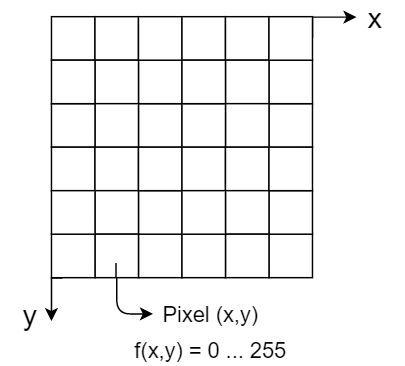
\includegraphics[width=0.9\textwidth]{images/imagembew.png}
    \caption{Modelo de imagem digital preto e branco}
  \end{minipage}
  \hfill
  \begin{minipage}[b]{0.45\textwidth}
    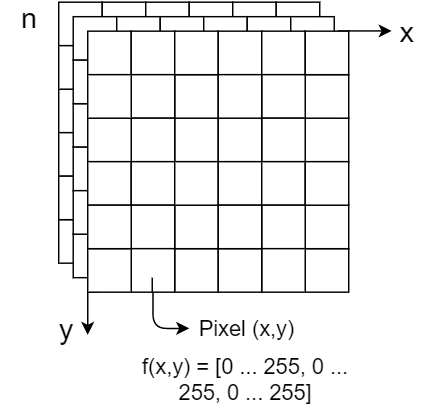
\includegraphics[width=0.9\textwidth]{images/imagemcolorida.png}
    \caption{Modelo de imagem digital colorida}
  \end{minipage}
  \caption{Representação de imagens digitais.}
  \label{fig:repre-imgs}
\end{figure}

\subsection{Filtragem Espacial de Imagens Digitais}

O processo de filtragem de uma imagem digital refere-se ao processo de transformação dos valores de intensidade dos pixels a partir dos seus vizinhos, dando assim origem a uma nova imagem. A filtragem é feita a partir da operação da convolução digital aplicando um \textit{kernel} --- matriz de tamanho 3x3, 5x5 ou 7x7 geralmente --- fixo sob todos os pixels da imagem com propósito de extrair características específicas da imagem, por exemplo, detecção de bordas, projetando-as na nova imagem \cite{stanford}.

Um exemplo intuitivo para entendimento é a média móvel, filtro que torna o valor de um pixel central a média dos seus oito pixels vizinhos. Definido matematicamente como $g[m,n] = \frac{1}{9} \sum_{i= -1}^{1} \sum_{j= -1}^{1} f[m - i,n - j]$ e ilustrado na Figura \ref{fig:blur}, a média móvel suaviza as bordas marcantes de uma imagem, criando um efeito de borrão sob a mesma \cite{stanford}.

\begin{figure}
    \centering
    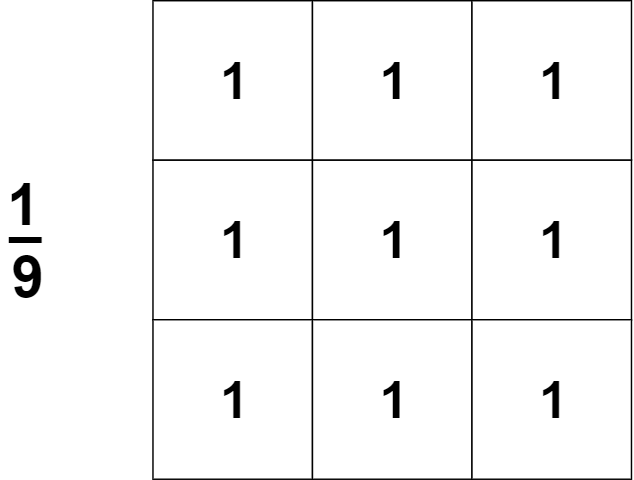
\includegraphics[width=0.35\textwidth]{images/blur.png}
    \caption{Kernel 3x3 da média móvel.}
    \label{fig:blur}
\end{figure}

\subsubsection{Operação da convolução}

Como mencionado, esta operação usa informação de pixels vizinhos em conjunto com um \textit{kernel} para transformar a intensidade de um pixel alvo. GoodFellow \textit{et al.} \cite{Goodfellow} ilustra este conceito a partir de um laser mantendo a localização de um nave espacial. O laser fornece uma única saída $x(t)$, a posição da nave no tempo $t$, podendo ser lido a qualquer instante de tempo. Agora imagina-se que o laser está em uma região ruidosa, para obtenção de uma estimativa menos ruidosa da posição é interessante fazer uma média de várias medições recentes. Para priorizar medidas recentes, esta média precisa associar estas a um peso maior, fazendo assim uma média ponderada $w(a)$, com a idade da medição. Se esta operação é aplicada a cada momento, é obtido uma função \textit{s} que fornece uma posição suavizada da espaçonave:

\begin{equation}
    s(t) = \int x(a)w(t - a)da
\end{equation}

Esta operação linear é denominada portanto convolução, por padrão escrita pelo símbolo * da forma $s(t) = (x * w) (t)$ \cite{Goodfellow}.

No exemplo ilustrativo acima \textit{w} precisa ser uma função densidade de probabilidade válida e 0 para todos os argumentos negativos, não valendo para o futuro. Ainda, o tempo válido para qualquer instante não é realístico. Esta operação, se feita em um computador, terá seu tempo discretizado, isto é, o sensor enviaria dados apenas em um intervalo regular de tempo. Pode-se assumir ainda que o tempo de medição é valido para valores inteiros, assim com \textit{x} e \textit{w} definidos apenas para \textit{t} inteiro. A convolução discreta pode ser escrita como \cite{Goodfellow}:

\begin{equation}
    s(t) = (x*w)(t) = \sum_{a = -\infty}^\infty x(a)w(t - a)
\end{equation}

A convolução discreta pode ser vista portanto como uma multiplicação de matrizes, sendo a matriz \textit{kernel} de valores fixos e variante no espaço da outra matriz. Este processo é ilustrado na Figura \ref{fig:convo} --- utilizando a terminologia de redes neurais convolucionais (Seção 2.2.2) --- onde o primeiro argumento da convolução (nosso \textit{x} do exemplo) refere-se uma imagem a ser filtrada, \textit{input}, o segundo argumento (a função \textit{w}) ao \textit{kernel} e a saída a mapas de características (do inglês, \textit{output} e \textit{feature maps}). Dessa forma, o \textit{kernel} desloca-se pela imagem fazendo operações de multiplicação e soma que resultarão numa imagem nova  \cite{Goodfellow}.

\begin{figure}
    \centering
    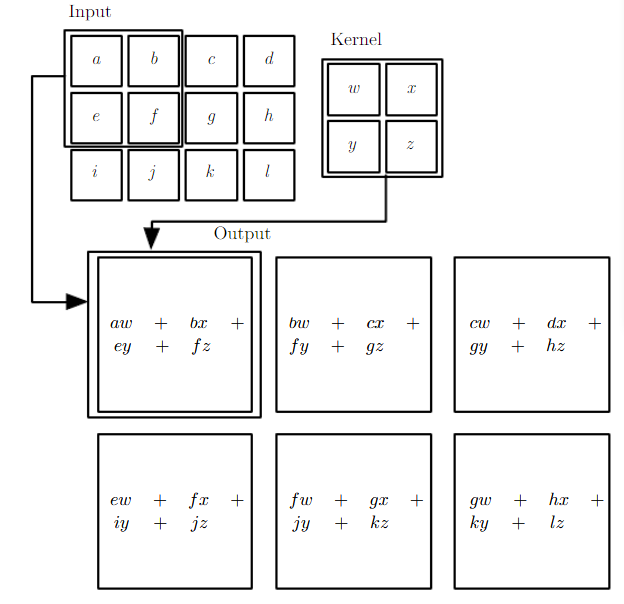
\includegraphics[width=0.65\textwidth]{images/convo.png}
    \captionsource{Um exemplo de convolução 2-d. As setas apontam para o resultado de uma única operação de convolução, sobre a parte superior esquerda da imagem, ao qual utiliza 4 pixels para gerar apenas um novo.}{ \protect\cite{Goodfellow}}
    \label{fig:convo}
\end{figure}

No exemplo a operação varre todos os pixels do \textit{input} de tamanho 4x3 com um \textit{kernel} de tamanho 2x2, resultando em uma imagem 3x2. Para detecção de características significantes em uma imagem é melhor que o \textit{kernel} não varra todos os pixels da imagem (técnica chamada interações esparsas, do inglês \textit{Sparse Interactions}) e ainda, a redução da resolução da imagem de saída se comparado com a entrada se faz benéfico para sistemas de visão computacional em geral e será melhor discutido na sessão de redes neurais convolucionais \cite{Goodfellow}.

\subsection{Segmentação de Imagens Digitais}

Segmentação de imagens é o processo de categorizar cada pixel em uma imagem, tal que pixels com o mesmo rótulo possuam a mesma propriedade semântica \cite{ghosh}. Humanos conseguem fazer segmentação de pixels de forma intuitiva, por exemplo, para uma imagem de rua saber qual região de pixels corresponde a rua, pessoas ou carros. Porém, para um computador conseguir atribuir significado a pixels juntos leva-se um pouco mais de esforço \cite{stanford}.  

A segmentação de imagens digitais pode ser entendido como uma evolução natural de classificação de imagens, esta que consiste em um afirmar para uma imagem inteira qual classe ela pertence ou é representada dentre algumas opções pré-estabelecidas. Localização e detecção são os passos seguintes para o aperfeiçoamento desta visão computacional, percebendo informações adicionais sobre o posicionamento espacial dos elementos na imagem. Naturalmente, após conseguir detectar elementos no espaço, surge a segmentação semântica, a categorização de todos os pixels em classes. Por fim, o maior nível de aperfeiçoamento consiste da segmentação de instâncias, também classificação de todos os pixels, porém com distinção de objetos de uma mesma classe, como representados na Figura \ref{fig:seg} \cite{garcia-garcia}.

\begin{figure}
  \centering
  \begin{minipage}[b]{0.4\textwidth}
    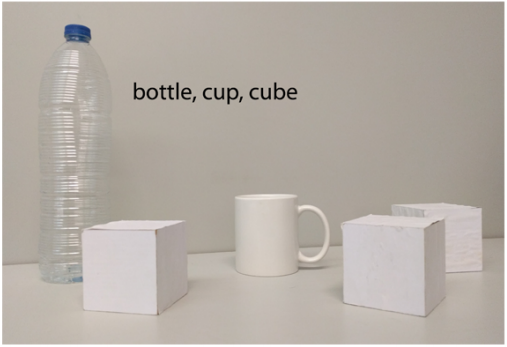
\includegraphics[width=\textwidth]{images/seg1.png}
    \caption{Classificação da imagem}
    \label{fig:seg}
  \end{minipage}
  \hfill
  \begin{minipage}[b]{0.4\textwidth}
    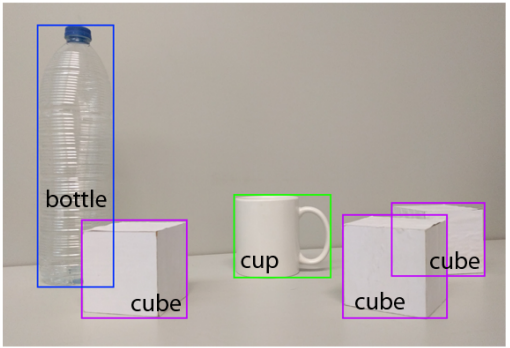
\includegraphics[width=\textwidth]{images/seg2.png}
    \caption{Localização de objetos}
    \label{fig:seg2}
  \end{minipage}
    \hfill
  \begin{minipage}[b]{0.4\textwidth}
    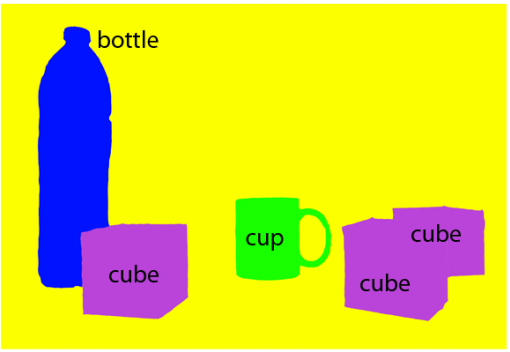
\includegraphics[width=\textwidth]{images/seg3.png}
    \caption{Segmentação semântica}
    \label{fig:seg3}
  \end{minipage}
    \hfill
  \begin{minipage}[b]{0.4\textwidth}
    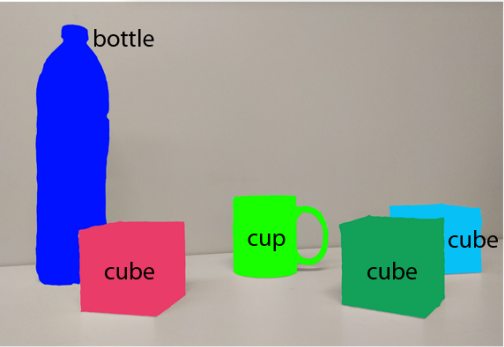
\includegraphics[width=\textwidth]{images/seg4.png}
    \caption{Segmentação de instâncias}
    \label{fig:seg4}
  \end{minipage}
  \captionsource{Evolução de níveis de entendimento de cenário por uma visão computacional: Classificação, detecção ou localização, segmentação semântica e segmentação de instância.}{ Adaptado de \protect\cite{garcia-garcia}} 
  \label{fig:seg}
\end{figure}

Segmentação atualmente é muito desejada de forma automática, onde dada uma grande quantidade de imagens obtidas de formas diversas, que um sistema inteligente consiga atribuir significado as imagens e torná-las ábil para uso. No contexto da moda, digamos que dada uma imagem de uma pessoa admirada deseja-se analisar seus sapatos, por exemplo. Estes muito provavelmente irão ocupar apenas uma pequena parte da imagem, fazendo com que maior parte da foto seja irrelevante para esta aplicação. Dessa forma, para um modelo inteligente aprender a segmentar de forma rápida e eficiente é necessário treiná-lo com ajuda de uma grande quantidade de imagens com alta qualidade de anotações.

Anotações de imagens é a forma de associar uma imagem ou uma seção de uma imagem com um identificador categórico de forma que um humano consiga informar a um modelo inteligente como perceber aquela imagem para idealmente aprender por exemplos. Dentre as várias formas de anotar uma imagem, destacam-se para este trabalho as caixas delimitadoras (Figura \ref{fig:seg2}), polígonos e segmentação semântica (Figura \ref{fig:seg3}). Caixas delimitadoras, consistem de retângulos delimitando as bordas do objeto, enquanto que polígonos suprimem quando os objetos não cabem dentro de uma caixa e precisam ser delimitados por uma forma geométrica mais complexa. Por último, as anotações de instâncias se faz a nível de pixel, determinando para cada pixel do objeto que ele pertence a uma certa classe \cite{anno}.

Técnicas para segmentação de cenas digitais não são recentes, porém sua popularidade foi revolucionada pelo aprendizado de máquina profundo. As fundamentadas em redes neurais convolucionais \ref{cnn} permitiram que esta área da visão computacional fosse aplicada de diversas formas no cotidiano, como em carros autônomos, iteração homem máquina, na busca de imagens inteligente e em realidade aumentada, para nomear algumas\cite{garcia-garcia}. 

\subsection{Redução de Dimensionalidade}

A redução de dimensionalidade consiste de uma área de estudo capaz de transformar representações de dados ao reduzir a quantidade de características descritivas destes, com o objetivo de buscar melhorar a performance de algoritmos de visão computacional, assim como de modelos baseados em aprendizado de máquina em geral \cite{stanford}. Dentre os métodos existentes, destacaremos aqui a Análise de Componentes Principais (do inglês, \textit{Principal Component Analysis} - \ac{PCA}) e \textit{t-Distributed Stochastic Neighbor Embedding} (\ac{t-SNE}).

\subsubsection{Análise de Componentes Principais}

Se imaginar um conjunto de características descrevendo dados alvos de estudo após um processamento de visão computacional e sabendo que usar todas as características não se mostra uma solução ótima devido o comprometimento de performance computacional e capacidade de aprendizado de modelos inteligentes, a dúvida que surge é: qual destas características devem ser priorizadas e quais destas podem ser removidas sem perder informações importantes?

Se as características fossem estatisticamente independentes, bastaria eliminar as menos relevantes, porém na prática muitas características dos dados são dependentes entre si, fazendo com uma única característica possa representar múltiplos tipos de informação. \ac{PCA} surge como uma possível solução para este problema, realizando uma transformação do espaço das características para obter informações descorrelacionados em um novo sistema de coordenadas \cite{dummy}.

De forma intuitiva \ac{PCA} pode ser pensado da seguinte forma: Digamos que é desejado diferenciar ingredientes de comida baseando-se em seus componentes nutricionais. Qual variável será suficientemente boa para diferenciar? Se a variável varia muito de um ingrediente para outro, será possível isolar bem os ingredientes, enquanto que mais difícil caso contrário. Quando os dados não apresentam uma variável que os separe bem, pode ser criado uma variável artificial a partir de combinações lineares de variáveis originais. Essencialmente \ac{PCA} acha a melhor combinação linear das variáveis originais para que a variância com relação a nova variável seja máxima \cite{paperspace}.

\begin{figure}
  \centering
  \begin{minipage}[b]{0.4\textwidth}
    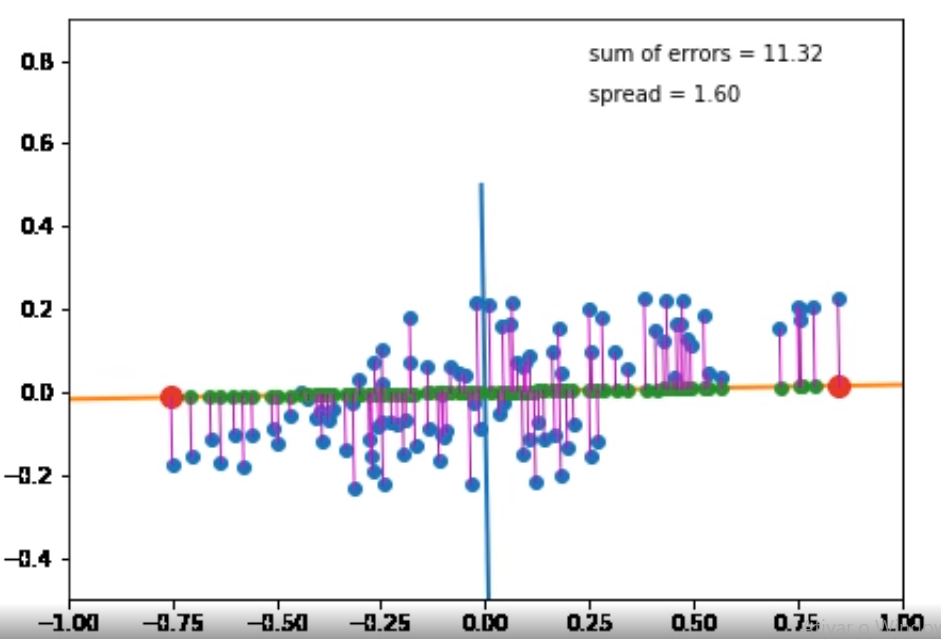
\includegraphics[width=\textwidth]{images/1.png}
    \caption{Autovalor = 11,32}
  \end{minipage}
  \hfill
  \begin{minipage}[b]{0.4\textwidth}
    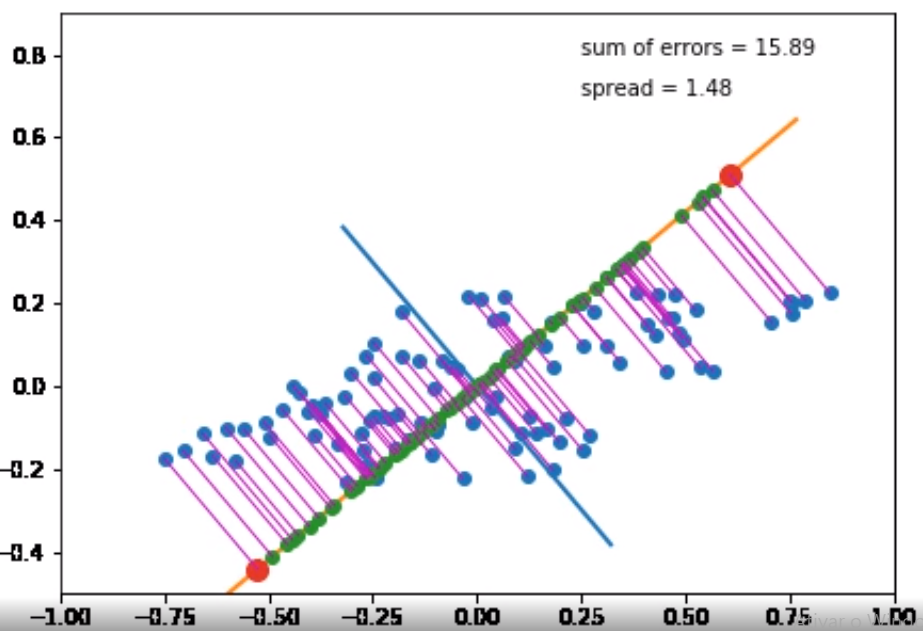
\includegraphics[width=\textwidth]{images/2.png}
    \caption{Autovalor = 15,89}
  \end{minipage}
    \hfill
  \begin{minipage}[b]{0.4\textwidth}
    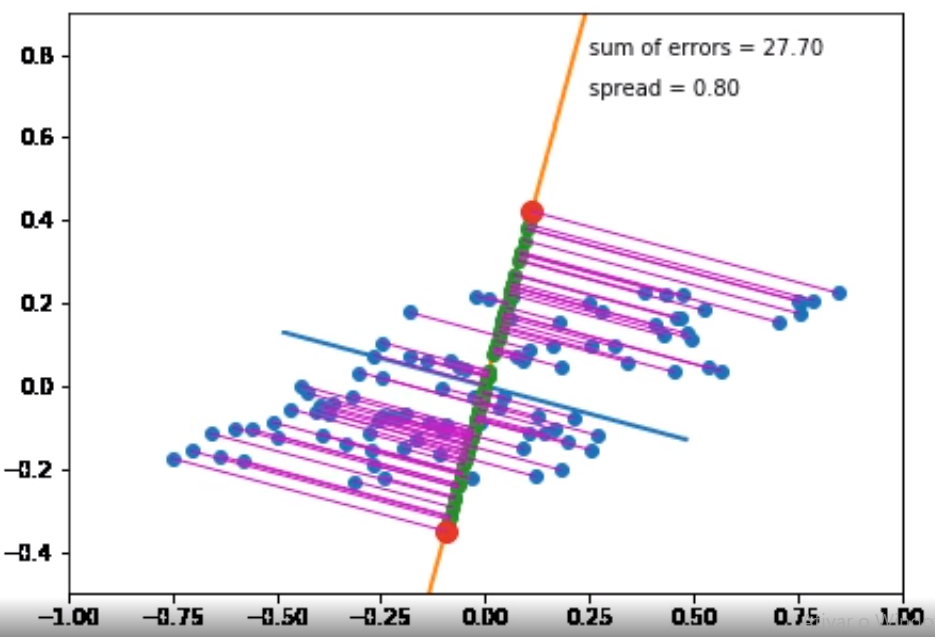
\includegraphics[width=\textwidth]{images/3.png}
    \caption{Autovalor = 27,70}
  \end{minipage}
    \hfill
  \begin{minipage}[b]{0.4\textwidth}
    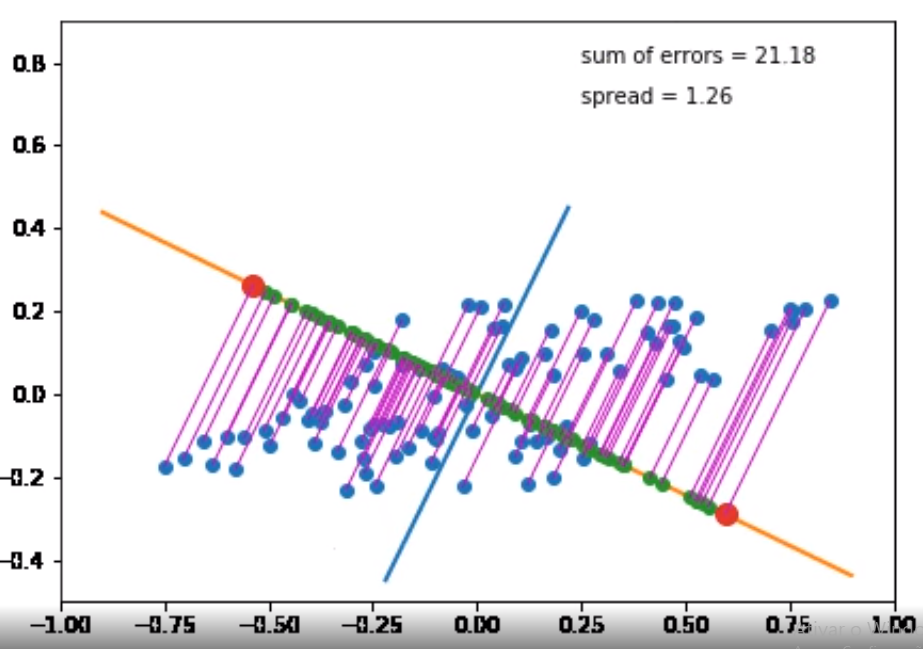
\includegraphics[width=\textwidth]{images/5.png}
    \caption{Autovalor = 21,18}
  \end{minipage}
  \captionsource{Ilustração de um vetor variando no espaço em busca da maior variância do dados projetados sobre si.}{ \protect\cite{paperspace}}
  \label{fig:animacao_pca}
\end{figure}

A Figura \ref{fig:animacao_pca} ajuda a ilustrar a técnica bidimensionalmente para fins de explicação, muito embora esta seja aplicada para qualquer número de dimensões que um conjuntos de dados venha a ter. Cada ponto azul representa um ponto de informação qualquer representado pelas coordenadas (x,y) (autovetor). Ao centralizar os dados no centro de dois eixos (x, y), são desenhados eixos aleatórios (linha laranja na imagem) passando pela origem, de forma a melhor representar os dados. Para saber o quão bom um eixo representa os dados, estes são projetados sobre o eixo (os pontos verdes) e são medidas as distância de cada ponto projetado para o centro do eixo (x, y) (autovalor). Eixos são aleatóriamente traçados passando pela origem de forma a maximizar o somatório dessas distâncias quadradas, que após achado será considerado um componente principal (PC1). Uma forma de entender o que este eixo está medindo é analisar a inclinação do PC1, que por exemplo, caso 0,25, significa que para cada 4 unidades que são percorridas no eixo x, uma unidade é percorrida no eixo y, em outras palavras  que os dados estão mais espalhados no eixo x, fazendo de x um eixo mais importante para descrever o espalhamento dos dados \cite{starQuest}.

Uma vez achado PC1, segue-se para achar outros componentes principais. No exemplo 2-d, PC2 será necessariamente perpendicular a PC1, também passando pela origem. Quando achados todos os componentes principais (determinados pelo usuário), os dados são então proejtados sobre esses novos eixos, ao invés do (x, y) originalmente centralizados e rotacionados para que os novos eixos fiquem alinhados com os (x,y) antigos. Os novos pontos dos dados serão então a combinação das coordenadas dos pontos projetados nesses eixos (pontos verdes), por isso a rotação, pois digamos que no PC1 um ponto está em (-4, 0) e em PC2 em (0, -1),  o dado real representado pela nova representação do PCA será em (-4, -1) \cite{starQuest}. 

A redução de dimensões em si acontece após o cálculo da variação para os componentes principais. Ao obter todos os autovalores para todos os componentes principais, consegue-se obter a variação para o PC através da divisão do autovalor pelo número de amostras - 1. Para o caso de dois eixos, digamos que a variação para PC1 = 15 e para PC2 = 3. Significa que 15+ 3 = 18, 15/18 = 83\% para PC1 e 3/18= 17\% para PC2 representa o quão este eixo de componente principal detém de informação sobre os dados. Para dados multidimensionais, ao calcular muitos PC's, a porcentagem de relevância tenderá a diminuir com o aumentar dos eixos, fazendo que a utilização de menos eixos resulte em dados informativos e com menos dimensões \cite{starQuest}. 

Neste trabalho \ac{PCA} será utilizado para reduzir dimensão de características descritivas obtidas por redes neurais para imagens digitais de moda. Na próxima seção será falado como redes neurais convolucionais leem características de imagens digitais e geram essa representação em alta dimensão, que para serem utilizadas em um algoritmo que classifique estas imagens se faz necessário reduzir a quantidade de dimensão e tentar descartar eventuais dados irrelevantes. 

\subsubsection{Distância do Cosseno}

Uma técnica comum aplicada a dados vetoriais é verificar sua similaridade ou dissimilaridade entre vetores, podendo ser utilizada a métrica da similiradidade ou distância do cosseno. Após aplicar o PCA, os vetores de características se tornam apteis a análises e uma forma muito eficiente de verificar relação entre vetores de dados, logo quais imagens são entendidas como semelhantes baseanda em características obtidas, é aplicando a métrica inversa da similaridade do cosseno.

A similaridade do cosseno é uma medida entre dois vetores não nulos A e B derivada da definição de definição do produto interno Euclidiano:

\begin{equation}
    A.B = ||A|| ||B||.\textit{cos}(\theta)
\end{equation}

levando a similaridade

\begin{equation}
    sim(\theta) = \textit{cos}(\theta) = \frac{A.B}{||A|| ||B||} = \frac{\sum_{i=1}^{n}A_iB_i}{\sqrt{\sum_{i=1}^{n}A_i^2}\sqrt{\sum_{i=1}^{n}B_i^2}}
\end{equation}

Essa medida de orientação, tem resultado de similaridade igual a 1 para vetores com a mesma orientação, 0 para vetores ortogonais e -1 para vetores completamente opostos, independente de suas magnitudes \cite{cosine}. Fazendo 1 - similaridade, portanto, é obtido uma métrica de distância do cosseno que mede a dissimilaridade e pode ser aplicada para medir a distância de semelhança entre imagens para um sistema de visão computacional.

\subsubsection{\textit{t-Distributed Stochastic Neighbor Embedding} (\ac{t-SNE})}

Técnicas de visualização são essenciais para o entendimento em aplicações com muitos dados, entretanto a maioria das técnicas de visualização podem somente serem aplicadas para inspeção de um número limitado de variáveis de interesse simultaneamente, muitas não sendo aplicáveis a dados multidimensionais. Uma forma efetiva de visualizar dados multidimensionais é representar cada objeto de informação como um ponto bidimensional visualizável, de forma tal que informações semelhantes sejam representadas por pontos próximos no espaço e dados não similares representados por pontos distantes \cite{techtalk}.

\begin{figure}
    \centering
    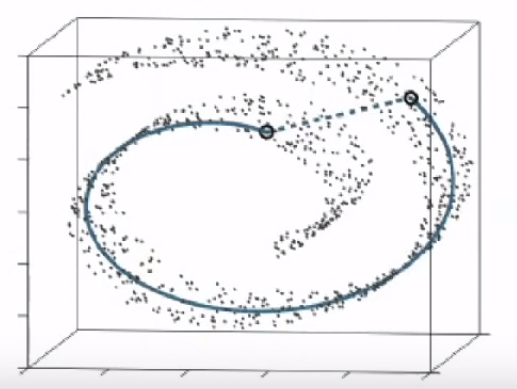
\includegraphics[width=0.35\textwidth]{images/pca.png}
    \caption{Comparação de amostras no espaço por distância (linha tracejada) e por contexto (pontos azuis).}
    \label{fig:pcaxtsne}
\end{figure}

Na figura \ref{fig:pcaxtsne} se considerarmos a distância entre amostras para media sua correlação, assim como PCA faz, forneceríamos um entendimento errôneo para a visualização, pois o mais importante para medir correlação nesta imagem é sua forma. Por conta deste problema da distância PCA não serve para visualização, na imagem os pontos seriam semelhantes devido a posição, porém se olharmos para a estrutura eles são muito diferentes \cite{techtalk}.

A técnica mais eficiente para embutir dados multi-dimensionais em uma visualização bidimensional ou tridimensional é abreviada por \ac{t-SNE}. Esta mede em altas dimensões similaridade entre pontos de forma a olhar apenas similaridade locais entre pontos próximos através da mimização de uma função que meça a discrepância entre as similaridades nos dados originais e nos dados mapeados. Exemplificando, a partir de uma distribuição gaussiana sobre os pontos da Figura \ref{fig:xdto2d}, um ponto alvo, o vermelho, tem sua densidade $x_i$ medida assim como seus vizinhos $x_j$ para serem aplicadas na equação:

\begin{equation}
    p_{ij} = \frac{exp(-||x_i - x_j||^2 /2\sigma^2)}{\sum_k\sum_{l\neq k}exp(-||x_k - x_l||^2/2\sigma^2)}
\end{equation}

Essa equação fornece então probabilidades, dado dois pontos \textit{i} e \textit{j}, essencialmente dizendo se dois pontos estão próximos (similares) em alta dimensão, para valores altos de $P_{ij}$, ou o contrário, para valores baixos \cite{techtalk}.

Para a baixa dimensão os pontos são distribuídos no plano como mostra a Figura \ref{fig:xdto2d} e aplicados a mesma lógica de similaridade, porém agora sobre a equação: 

\begin{equation}
    q_{ij} = \frac{(1 + ||y_i - x_j||^2)^{-1} }{\sum_k\sum_{l\neq k}(1 + ||y_i - x_j||^2)^{-1}}
\end{equation}

de forma que as probabilidades $q_{ij}$ e $p_{ij}$ sejam semelhantes, garantindo que a representação dos pontos em alta e baixa dimensão são semelhantes. A medida de semelhança entre as equações é feita pela divergência Kullback-Leibler:

\begin{equation}
    KL(P||Q) = \sum_i\sum_{j\neq i} = p_{ij}log\frac{p_{ij}}{q_{ij}}
\end{equation}

Portanto, os pontos em baixa dimensão são alternados e otimizados a partir do gradiente descendente de forma a minimizar a divergência Kullback-Leibler.

\begin{figure}
    \centering
    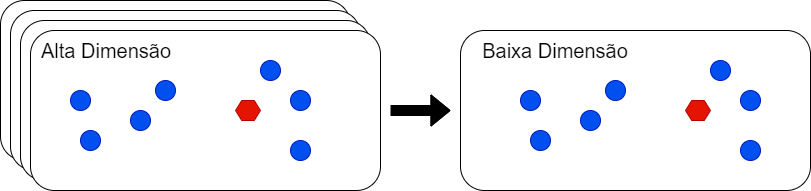
\includegraphics[width=0.8\textwidth]{images/xdto2d.png}
    \captionsource{Mapeamento de dados de alta dimensão para baixa dimensão preservando a densidade de distribuição das amostras.}{ Adaptado de \protect\cite{techtalk}}
    \label{fig:xdto2d}
\end{figure}

Van der Maaten, autor da técnica, ilustra seu potencial para imagens a partir de amostras de números. Após processar as imagens através de um modelo inteligente obtém-se uma grande quantidade de características descritivas para cada amostra. A técnica é utilizada portanto para visualização em duas dimensões das características em altas dimensões. A Figura \ref{fig:tsne} ilustra o resultado obtido onde todas as amostras de imagens referentes a um número são visualizadas próximas de si, com distância para as outras amostras de acordo com a similaridade dos números \cite{techtalk}.

\begin{figure}
    \centering
    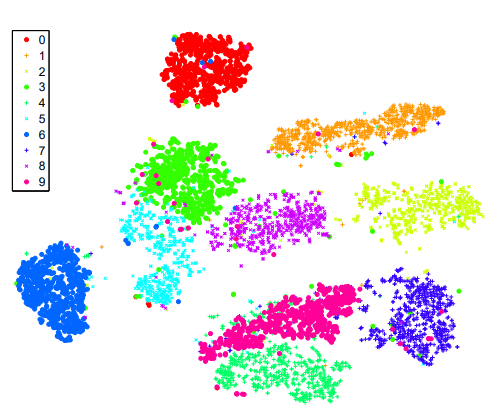
\includegraphics[width=0.6\textwidth]{images/ts.png}
    \captionsource{Exemplo de visualização utilizando t-SNE aplicado a imagens de número. Este não só mostra as diversas amostras de imagens aglomeradas por classe como também preserva em duas dimensões a distância entre as classes baseando-se em suas características descritivas.}{ \protect\cite{techtalk}}
    \label{fig:tsne}
\end{figure}

Como intuitiamente explicado pela equipe do "Google Brain" \cite{distill}, t-SNE ilustra algumas regalias com a técnica. Primeiro um fato essencial para análise dos resultados é que o melhor resultado deve ser achado por meio de múltiplos plotes e tentativas. Devido o algoritmo não produzir resultados similares em tentativas sucessivas, há hiperparâmetros do processo de otimização a serem tunados para que o usuário encontre um resultado satisfatório. Outro ponto interessante é que o tamanho dos aglomerados não significa nada, pois o algoritmo adapta a noção de distância para a varição de distâncias regionais, não visualizáveis nos plotes. Em alguns casos, dependendo dos hiperparâmetros e dos dados, a distância entre os aglomerados pode não significar nada. Devido a complexidade dos dados da vida real e a quantidade de aglomerados e número de elementos, o algoritmo pode não chegar a uma distância ótima. Portanto, t-SNE é uma técnica que exige testes e entendimento de parâmetros para ser melhor utilizada e quando em casos simples pode levar ao desenvolvimento de intuição do que está acontecendo ---  de forma contrátia pode levar a deduções errôneas.

\section{Aprendizado de Máquina}

Algoritmo de aprendizado de máquina são algoritmos capazes de aprender a partir de dados. No seu livro clássico, Mitchell (1997) define aprendizado como um programa de computador que ao ter aprendido a fazer tarefas T com performance P baseado em uma experiência E, consiga melhorar sua performance P em T a partir desta experiência E. Aprendizado aqui é o sentido atribuído ao alcance da habilidade de performar a tarefa \cite{Goodfellow}.

Em aprendizado de máquina o objetivo é fazer com que os algoritmos --- também chamados de modelos --- generalizem seu aprendizado, por meio de um conjunto de dados prévio, em dados nunca antes visto. Os dados a serem fornecidos ao modelo para treinamento devem ser preferencialmente separados em três conjuntos: Treinamento, validação e teste \cite{chollet}. O subconjunto de validação é obtido a partir do subconjunto treinamento --- em torno de 70\% de todos os dados ---  a partir de proporções geralmente próximas a 80\% para treinamento e 20\% para validação. A primeira porção é utilizada para regular os parâmetros do modelo no processo de aprendizado, enquanto que o segundo conjunto usado para estimar a generalização durante o treinamento, permitindo que o modelo se adeque de forma a melhorá-la. Quando o modelo finaliza seu processo de aprendizado, pode ser testado utilizando os 30\% de dados para teste, sendo importante que os dados para cada conjunto sejam escolhidos de forma bem distribuída, para que o modelo em seu processo de aprendizado experiencie todos os tipos de exemplos, assim como seja testado sob as mesmas condições \cite{Goodfellow}.  

Os diversos algoritmos de aprendizado de máquina podem ser amplamente categorizado como supervisionado e não supervisionado a partir da experiência que estes têm durante o processo de aprendizado. O aprendizado supervisionado é baseado em dados categorizados, associados a um rótulo, por exemplo, se os dados de flores são classificáveis em três tipos, um modelo pode ser treinado para que possa diferenciar flores quanto a seus tipos. Por outra via, o aprendizado não supervisionado baseia-se no aprendizado de características importantes da estrutura dos dados apresentados. A classificação pode ser feita agrupando os dados que apresentem características semelhantes, porém o modelo precisa aprender esta relação \cite{Goodfellow}.

O desafio de generalizar o aprendizado para novos exemplos se torna exponencialmente mais difícil quando utiliza-se dados multidimensionais e como os mecanismos usados para conseguir generalizar funções multdimensionais em aprendizado de máquina tradicional são insuficientes, desenvolveram-se técnicas de aprendizado de máquina profundo (do inglês, \textit{Deep Learning}). Portanto, aprendizado de máquina profundo permite o computador construir conceitos complexos a partir de conceitos mais simples:

\begin{adjustwidth}{2.5em}{}

"Aprendizado profundo é um tipo particular de aprendizado de máquina que conquista grande poder e flexibilidade por aprender a representar o mundo como uma hierarquia entrelaçada de conceitos, com cada conceito definido em relação a conceitos mais simples e representações mais abstratas computadas em termos dos menos abstratos" \cite{Goodfellow}.

\end{adjustwidth}

Nessa seção serão introduzidos técnicas específicas do campo \textit{deep learning} utilizadas em visão computacional, tais como redes neurais convolucionais e \textit{Mask} R-CNN. 

\subsection{Redes Neurais Artificiais}

Redes neurais artificiais são consideradas por excelência o exemplo de qualidade dos modelos de aprendizado profundo. Este modelo matemático é chamado de rede devido sua representação composta de um emaranhado de diferentes funções conectadas entre si. Por exemplo, se houverem três funções $f^{(1)}$, $f^{(2)}$, $f^{(3)}$ conectadas em uma corrente para formar $f(x) = f^{(3)}(f^{(2)}(f^{(1)}(x)))$, a $f^{(1)}$ é chamada de primeira camada da rede, $f^{(2)}$ a segunda camada e assim por diante. O total de camadas de uma rede mede a profundidade do modelo \cite{Goodfellow}.

Este conceito de modelo matemático pode ser aplicado em diferentes arquiteturas, porém todas com um objetivo em comum, de aproximar uma função $f^*$. Exemplificando, para gerar um classificador $y = f*(x)$ que mapeia uma entrada a uma determinada categoria, a rede neural consegue definir uma função $y = f(x;\theta)$ e a partir dos dados aprender qual o valor de $\theta$ que resulta no melhor classificador \cite{Goodfellow}.

Estas estruturas de rede têm "neural" em seu nome devido a inspiração biológica com relação ao funcionamento do cérebro. Entretanto, o objetivo destas não deve ser pensado como de modelar o cérebro perfeitamente e sim como máquinas de aproximação de funções que são criadas para conquistar generalização estatística, ocasionalmente podendo levar a um paralelo com o que sabemos sobre nosso cérebro \cite{Goodfellow}.

\subsection{Redes Neurais Convolucionais} \label{cnn}

Redes neurais convolucionais, comumente chamadas de \ac{CNN} (do inglês, \textit{Convolutional Neural Networks}), são um tipo de rede neural especializada para processamento de dados em formato de grade que têm obtido extremo sucesso em aplicações práticas diversas, em destaque utilizando imagens digitais. Goodfellow \textit{et al.} em seu livro define esta rede como "simplesmente um modelo de rede neural que aplica a operação matemática convolução no lugar de multiplicação de matriz básica em pelo menos uma de suas camadas" \cite{Goodfellow}.

A diferença fundamental entre camadas com funções totalmente conectadas e convolucionais está no modo do aprendizado. Camadas densas aprendem padrões globais, enquanto que camadas convolucionais aprendem padrões locais, como na Figura \ref{fig:quatro} mostra, padrões aprendidos são encontrados através de uma pequena janela 2-d \cite{chollet}. 

\begin{figure}
    \centering
    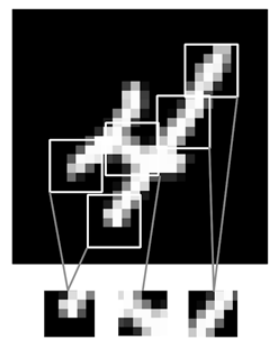
\includegraphics[width=0.2\textwidth]{images/covnet4.png}
    \captionsource{Imagens podem ser quebradas em padrões locais tais como bordas, texturas, entre outros.}{ \protect\cite{chollet}}
    \label{fig:quatro}
\end{figure}

Essa propriedade permite portanto que as \ac{CNN}'s tenham duas capacidades poderosas e importantes para este trabalho: Os padrões aprendidos são invariantes a sua translação e o aprendizado estabelece uma hierarquia espacial. Ao aprender um certo padrão, supondo que na borda inferior da imagem, a rede conseguirá reconhecer este em qualquer lugar que ele vier a aparecer; ainda, a primeira camada de convolução aprenderá padrões locais e pequenos, tais como bordas, enquanto que a segunda camada aprenderá padrões maiores feitos dos padrões da primeira camada e assim por diante até a rede como um todo consiga definir conceitos completos como detectar um animal, por exemplo \cite{chollet}.

As arquitetura de uma rede convolucional é composta de três camadas principais, chamadas camada de convolução, camada de pool e camada totalmente conectada. Ilustrada pela Figura \ref{fig:passaro}, uma imagem de entrada passa por uma série de camadas de convoluções composta por filtros, posteriormente camadas de pool até chegar por fim na camada classificatória, fornecendo uma classe para a imagem fornecida \cite{chollet}.

\begin{figure}
    \centering
    \includegraphics[width=0.8\textwidth]{images/cnn.png}
    \caption{Arquitetura básica de uma rede neural convolucional.}
    \label{fig:passaro}
\end{figure}

\subsubsection{Camadas de Convolução}

A principal funcionalidade das redes neurais convolucionais de aprender padrões e características acontece devido a operação de otimização aplicada aos filtros que performam a convolução da rede. Nessas camadas se constrói um mapa de características para a imagem de entrada a partir da série de convoluções aplicadas a imagem. As características obtidas dependem dos filtros aplicados, como já mencionado na seção 2.1.1, estes inicialmente aleatórios até serem otimizados pelo gradiente descendente em filtros que conseguem extrair exatamente o que o domínio de imagens exige; por exemplo, se houver necessidade da rede reconhecer um gato, dentre seus filtros terão os responsáveis por achar os olhos, pêlos, etc. \cite{chollet}. A figura \ref{fig:zero} ilustra um filtro sendo aplicado a uma imagem e seu resultado que composerá o mapa de características. 

\begin{figure}
    \centering
    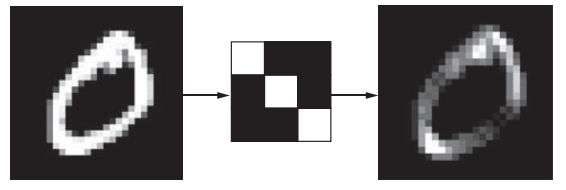
\includegraphics[width=0.45\textwidth]{images/zero.png}
    \captionsource{Resultado de uma operação de convolução.}{ \protect\cite{chollet}}
    \label{fig:zero}
\end{figure}

\subsubsection{Camadas de \textit{Pool}}

Estas camadas minimizam a quantidade de informação obtida pelas camadas de convolução de forma a torná-las mais relevantes. Esta operação é também é feita deslizando uma janela sobre a imagem, em busca geralmente dos maiores valores de pixel dentro da janela (figura \ref{fig:maxpool}). Por exemplo, se após a convolução obtém-se imagens de tamanho 26 x 26, a operação de \textit{max-pooling} diminuirá a mesma para 13 x 13 \cite{chollet}.

\begin{figure}
    \centering
    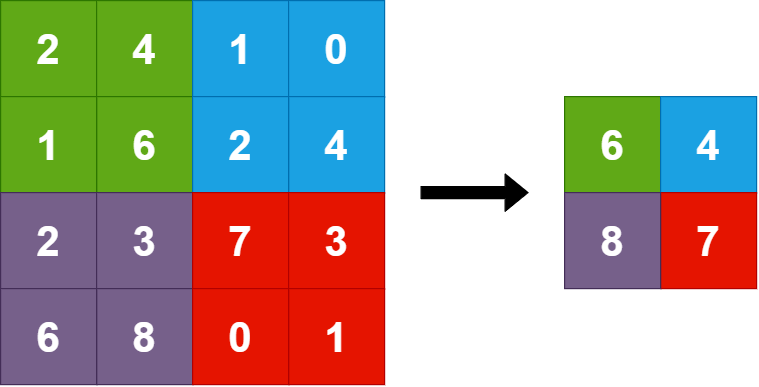
\includegraphics[width=0.4\textwidth]{images/maxpool.png}
    \caption{Operação de \textit{max-pooling}}
    \label{fig:maxpool}
\end{figure}

A motivação para reduzir a quantidade de amostras é reduzir o número de coeficientes do mapa de características a serem processados pela rede. Em poucas palavras, as características obtidas tendem a codificar a presença de algum padrão ou conceito, logo é mais informativo olhar sobre a máxima presença de diferentes características do que a média destas espalhadas em muitos valores \cite{chollet}.

\subsubsection{Camadas Classificatória}

Após uma série de camadas de convolução e de \textit{pool} a imagem se torna uma abstração com uma representação multidimensional de mapa de características. A partir deste é adicionado uma camada classificatória para fornecer uma resposta informativa ao usuário sobre todas as características abstratas. Esta etapa pode ser entendida como um modelo de aprendizado a parte que será treinado de acordo com a aplicação prática do modelo e performance desejada \cite{chollet}.

\subsubsection{Transferência de Aprendizado}

Uma prática comum e altamente eficiente em aplicações com redes neurais convolucionais que possuem pequeno conjunto de dados para treinamento é usar redes pré-treinadas, ao invés de treinar uma por completo. Esta técnica conta com \ac{CNN}'s  previamente treinadas sobre uma grande quantidade de dados, tipicamente para classificação de imagem em larga escala. Se o conjunto de dados fornecido para o treinamento for grande suficiente e abrangente suficiente, possibilitará que a hierarquia espacial das características aprendidas pela rede pré-treinada aja como um modelo genérico de visão do mundo, sendo úteis para diversas aplicações de visão computacional completamente diferentes da tarefa onde foram treinadas --- transferência de aprendizado (do inglês, \textit{Transfer Learning}) \cite{chollet}.

Há duas formas de utilizar redes pré-treinadas, para extração de características e para ajuste de rede, porém para este trabalho só será relevante o uso como extrator de características. Este método consiste em utilizar o aprendizado obtido de um treinamento prévio para extrair características de novas imagens, geralmente de um contexto diferente. As características obtidas --- mapas de características abstratos --- podem então alimentar um classificador que ao ser treinado para uma aplicação específica poderá ser usado para outro fim de sua base convolucional em comum (Figura \ref{fig:transfer}). 

\begin{figure}
    \centering
    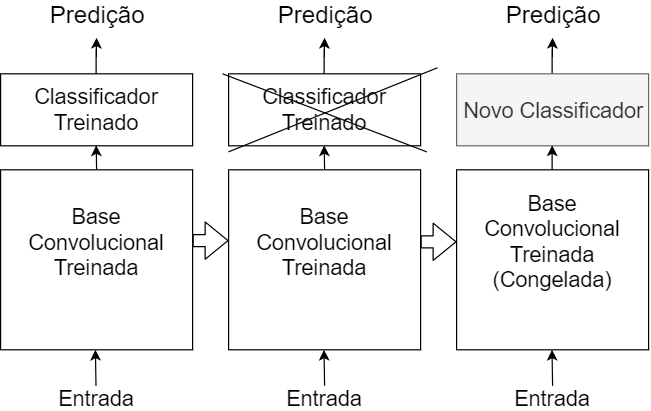
\includegraphics[width=0.7\textwidth]{images/transfer.png}
    \captionsource{Processo de alterar um modelo para utilização como transferência de aprendizado. A partir de um modelo composto de uma CNN e um classificado é retirado o classificador e colocado outro sobre a mesma base convolutiva, esta mantida sem alteração.}{ Adaptado de \protect\cite{chollet}}
    \label{fig:transfer}
\end{figure}

Em geral deve-se evitar reutilizar classificadores para diferentes aplicações, já que as representações aprendidas por esta camada são especificas da aplicação. Para utilizar a base convolutiva, que tem um potencial mais genérico e reutilizável, deve-se atentar para a profundidade das camadas na rede, pois as camadas mais fundas são mais especializadas e a extração de características para uma aplicação muito diferente pode ser comprometida se os dados novos diferem muito dos dados que esta foi treinada \cite{chollet}.

\subsection{\textit{Mask} R-CNN}

Partindo da renomada arquitetura R-CNN, do inglês, \textit{Regional Convolutional Neural Network}, esta arquitetura de rede neural foi recentemente (2019) introduzida como complemento do modelo mais renomado para detecção de objetos \textit{Faster} R-CNN. Nesta nova arquitetura foi introduzido o necessário para avançar na ordem de complexidade de segmentação e chegar a segmentação de instâncias. 

Segmentação de instâncias é desafiador pois requer uma detecção correta de todos os objetos em uma imagem enquanto ainda segmenta de forma precisa cada uma de suas instâncias. Esta técnica combina os elementos de detecção e classificação de objetos (Figura \ref{fig:seg}) e segmentação semântica \cite{maskrcnn}.

\begin{figure}
    \centering
    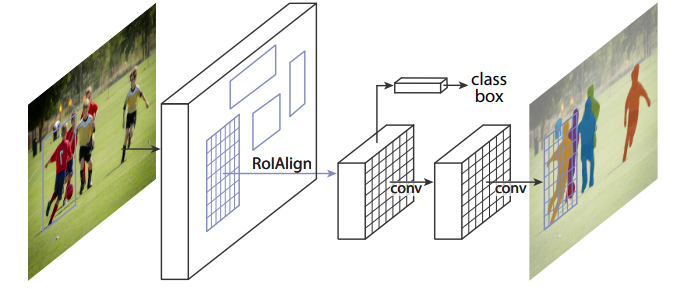
\includegraphics[width=0.6\textwidth]{images/futebol.png}
    \captionsource{Arquitetura da rede \textit{Mask} R-CNN}{ \protect\cite{maskrcnn}}
    \label{fig:futebol}
\end{figure}

A estrutura proposta pelo grupo de pesquisa com \ac{IA} do Facebook, ilustrada na Figura \ref{fig:futebol}, recebe uma imagem, detecta a região de interesse e de forma paralela classifica o objeto detectado ao mesmo tempo que melhora sua região delimitadora do objeto detectado (do inglês, \textit{Region of Interest Align} - RoIAlign). Após detectada com precisão a região de interesse este segmento da imagem é passado por uma rede neural convolucional totalmente conectada para prever a segmentação de máscara, pixel a pixel. Alguns exemplos de aplicação podem ser visto na Figura \ref{fig:mask}, onde para uma mesma classe, por exemplo "pessoa", a rede consegue distinguir diferentes elementos através de máscaras, e ainda delimitar seus limites com um retângulo demarcador \cite{maskrcnn}. 

\begin{figure}
    \centering
    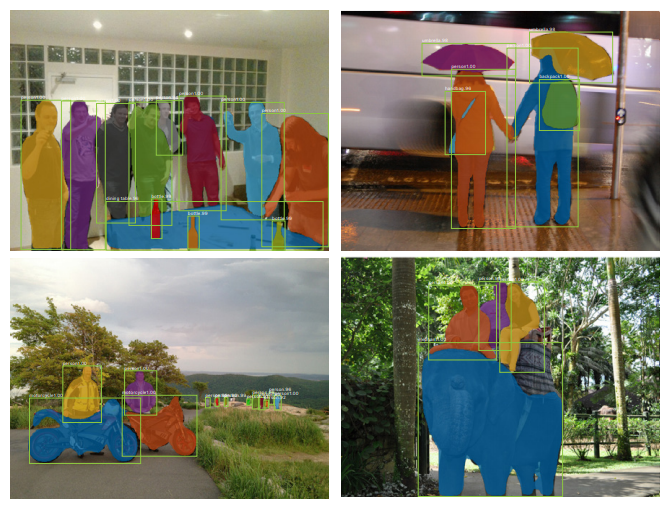
\includegraphics[width=0.6\textwidth]{images/mask.png}
    \captionsource{Exemplo de resultados obtidos pelo time desenvolvedor da \textit{Mask} R-CNN aplicado sobre o dataset COCO.}{ \protect\cite{maskrcnn}}
    \label{fig:mask}
\end{figure}

\chapter{Trabalhos Relacionados}
\label{cha:relacionados}

Há diferentes tarefas envolvendo análise de imagens de vestimentas, tais como detecção de roupas, predição de ponto chave, segmentação e obtenção de roupas (traduções livres do inglês, \textit{clothes detection}, \textit{landmark prediction}, \textit{clothes segmentation} e \textit{retrieval}) \cite{deepfashion2}. De acordo com um estudo apresentado por \cite{jia} a análise de vestimentas tem recebido um aumento de atenção contínuo da comunidade de visão computacional nesta década, marcando avançados significativos nas quatro áreas mencionadas.

Trabalhos pioneiros desenvolveram um processo padrão de processamento aperfeiçoado "à mão"  --- como é chamado devido a grande complexidade de parâmetros para calibrar --- enquanto os processos baseados em \textit{deep learning} não vinham à tona \cite{deephuman}. Serão mencionados alguns dos trabalhos importantes que marcaram esta trajetória, dando ênfase nos que vieram a dar suporte no desenvolvimento deste trabalho nos âmbitos de segmentação de vestimentas e análise de moda envolvendo imagens digitais. 

\section{Segmentação de Vestimentas e Conjuntos de Dados}

%"image retrieval" com cross domain porém: https://arxiv.org/pdf/1709.01784.pdf |||| http://citeseerx.ist.psu.edu/viewdoc/download?doi=10.1.1.370.6283&rep=rep1&type=pdf |||| https://ieeexplore.ieee.org/document/7805463 ||| http://www.nlpr.ia.ac.cn/2012papers/gjhy/gh94.pdf

%image search: https://winstonhsu.info/wp-content/uploads/2017/08/kuo17feature.pdf

%For example, WTBI [5] and DARN [7] have 425K and 182K images respectively. They scraped category labels from metadata of the collected images from online shopping websites, making their labels noisy. In contrast, CCP [20], DeepFashion [14], and ModaNet [21] obtain category labels from human annotators. (DeepFashion2)

Em 2012, \cite{Fashionista} foram pioneiros em aplicar técnicas clássicas de segmentação de imagens para treinar o modelo estatístico CRF para classificação de imagens de pessoas em 53 categorias de vestimentas possíveis. Tendo usado 685 imagens anotadas de pessoas exibindo o que vestiam para treino e teste, obtiveram 80.1\% de acurácia na análise de pixels e introduziram na literatura o primeiro conjunto de dados com imagens de vestimentas anotadas disponibilizado online, denominado "fashionista" --- suporte para diversos estudos subsequentes na área. %[20, 5, 7, 3, 14, 12, 21, CFPD, deepfashion2, runway2realway]

O famoso conjunto de dados "Paper doll" \cite{paperdoll}, buscando melhorar a acurácia sobre o "fashionista" , implementou descritor de estilo para buscar estilo de roupa semelhantes: um vetor de características descritivas para uma imagem, a partir de técnicas clássicas para extração de características como RGB, Lab, MR8, HOG, \textit{Boundary Distance}, e \textit{Pose Distance}. Também, observou a problemática da dimensão dos vetores de características para imagem e aplicou \ac{PCA} para reduzir a dimensão de 39.168 para 441 dimensões.

%magic closet [WoW dataset] - não usa CNN para features most suitable clothing by considering the wearing properly and wearing aesthetically principles. We adopted a latent SVM based recommendation model to incorporate the matching rules among visual feature, attribute and occasion within a unified framework. To learn and evaluate the model, we collected a large clothing dataset with full attribute and occasion annotations.

Em cima do "Paper doll" foram introduzidos diversos estudos com diferentes propostas, muitos dos quais trabalharam em cima de obtenção de imagem. Com grande potencial para vendas online, esta área busca encontrar imagens contendo vestimentas similares a uma determinada imagem, geralmente da rua para loja online. "Runway to Realway" \cite{runway2realway}, entretanto, foi além da busca por similaridade ao criar um dataset com 348.598 imagens de desfiles de moda em um período de 15 anos e aplicar o descritor de estilo para treinar um modelo de classificação capaz de medir similaridade entre roupas a partir da opinião humana. O mais atraente deste estudo se fez a capacidade dos descritivos não só acharem imagens semelhantes no banco de imagens, como também estudar a moda ao longo dos anos, percebendo variação de tendências com o tempo. 
%(deep human parsing, Human parsing Contextualized-CNN)

Não demorou para que as redes neurais tomassem de conta dos estudos desta área, melhorando a acurácia de seus precursores na segmentação e extração de características, assim como criando nossas possibilidades de aplicações. "Exact Street2Shop Dataset" \cite{wheretobuyit}, por exemplo, se destacou por ter coletado e categorizado 20.357 imagens de pessoas usando roupas no cotidiano e 404.683 de lojas online, onde 39.479 formavam pares de itens iguais. O estudo que treinou uma CNN para obtenção de características, usou humanos e IA para avaliar sua acurácia e mostrou bons resultado tendo medido a similaridade entre vetores de características através da distância do cosseno. \cite{parsing} também se destaca por utilizar o pequeno "fashionista" e chegar numa acurácia nível estado da arte a partir de uma rede pré-treinada no dataset "ImageNet". 

Os conjuntos de dados "ModaNet" \cite{modanet} e "DeepFashion2" \cite{deepfashion2} se mostram as opções mais recentes para fundamentar estudos de análises de moda. O primeiro, que consiste de uma coleção de 55.176 anotações humanas em imagens a nível de pixel, contendo pessoas em poses diversas e de boa resolução, sobrepõe anotações consideradas fracas do "Paper doll". Essa coleção de anotações feitas com imagens do "Paper doll" foi construída de forma a possibilitar testar os algoritmos estado da arte para detecção e segmentação sobre 13 categorias, que têm sido adotadas como de maior interesse para pesquisa e aplicações de mercado pelo mundo: bolsa, cinto, botas, calçados, sobretudo, vestido, óculos de sol, calças, superior, shorts, saia, chapéu e gravata/cachecol \cite{modanet}. Diferentemente de outros conjuntos de dados com anotações, "ModaNet" fornece anotações a nível de pixel sobre cada item de roupa para cada imagem formando um polígono delimitador para a categoria da anotação. 

\begin{table}[]
\centering
\begin{tabular}{@{}llll@{}}
\toprule
Categoria         & Descrição                      & Treino & Validação \\ \midrule
Bolsa             & Bolsa                          & 36.699 & 2.155     \\
Cinto             & Cinto                          & 13.743 & 771       \\
Botas             & Botas                          & 7.068  & 691       \\
Calçados          & Calçados                       & 39.364 & 1.617     \\
Sobretudo         & Casaco, jaqueta, terno, blazer & 23.743 & 1.358     \\
Vestido           & Vestido, camisão               & 14.460 & 804       \\
Óculos de sol     & Óculos de sol                  & 8.780  & 524       \\
Calça             & Calças, Calças jeans, leggings & 23.075 & 1.172     \\
Top               & Top, blusa, camiseta, camisa   & 34.745 & 1.862     \\
Shorts            & Shorts                         & 5.775  & 429       \\
Saia              & Saia                           & 10.860 & 555       \\
Chapéu            & Chapéu                         & 5.405  & 491       \\
Cachecol\&Gravata & Cachecol, gravata              & 3.990  & 378       \\ \bottomrule
\end{tabular}
\caption{Distribuiçao das categorias no banco de anotações "ModaNet"}
\label{table:estat}
\end{table}

"DeepFashion 2" \cite{deepfashion2}, por sua vez, foca em um construir uma ferramenta completa para entendimento de imagens de moda. Se auto considerado estado da arte atualmente, este é composto por 491.000 imagens anotadas com diferentes perspectivas, contendo não só anotações de pixels como também informações de zoom e \textit{landmarks}, por exemplo. Pela primeira vez na literatura é proposto o desafio de estimação de pose de roupas, estendendo o campo de estudo feito até agora sobre poses humanas. Prometendo melhorar a performance da análise de imagens de moda e aplicações no mundo real, este trabalho é pioneiro na estimação de poses de vestimentas com o chamado \textit{landmarks}, apresentando maior aproveitamento do que poses humanas. Ainda, apesar de fazerem uso extensivo da recente arquitetura "Mask R-CNN" e validarem seu benefício, propõem uma nova construída sobre esta, denominada "Match R-CNN". 

\section{Análise de Moda Através de Imagens Digitais}

% não consegui acesso Hidayati et al. analyze catwalk images from NYC fashion shows to find style trends in high-end fashion [2014].
 
Como mencionado acima, "Runway to Realway" \cite{runway2realway} partiu da estimação de pose e análise de vestimenta para concluir que alguns estilos de roupa como estampa floral tinha seu uso variado no tempo. Porém, surgiram estudos mais relevantes voltados para a análise da moda em si através de dados. "StreetStyle" \cite{streetstyle} procurou analisar moda e estilo de se vestir de milhões de imagens ao redor do mundo por um período de alguns anos. Utilizando aprendizado supervisionado e não supervisionado sobre um dataset próprio, procurou obter atributos de roupas de novas imagens e classificá-las através de aglomerados automáticos para rápida detecção de correlação (\ac{t-SNE}), permitindo análise no formato de mapa. Este trabalho que também utiliza \ac{PCA} para redução dos vetores de características, obtém bons resultados ao perceber padrões de vestimentas nas maiores cidades do mundo, porém com uma grande limitação das imagens utilizadas serem todas com enquadramento de busto e baixa resolução.

Assim como "StreetStyle", \cite{learningvisual} utilizou agrupamento automático no espaço para entender como sua rede entendia os dados de moda. \cite{geostyle}, por sua vez, desenvolveu um trabalho em cima do "StreetStyle" para analisar milhões de imagens e não só entender como as pessoas estavam se vestindo pelo mundo, mas prever eventos responsáveis por mudanças nos padrões, por exemplo, grande número de fotos publicadas com pessoas usando amarelo em 2014 ser relacionado na copa do mundo. 

Diferentemente, \cite{brands} buscou analisar associação entre marcas através de imagens digitais. Associação de marca, conceito do marketing, pode ser definido como atitudes ou sentimentos na mente do consumidor em relação a uma marca ou produto, por exemplo, "o que vêm a cabeça de um consumidor quando este pensa na marca Nike?". Esse estudo inovador, utiliza visão computacional no modelo clássico perfeccionado a mão (HSV, SIFT e HOG) para buscar similaridade entre imagens e segmentação do que representaria a marca dada uma determinada imagem. Mesmo tendo analisado quase 5 milhões de imagens de 48 marcas, o resultado mostra imagens em baixa resolução, não ficando claro como poderia servir de informação útil. 

\chapter{Desenvolvimento}

O desenvolvimento do trabalho segue uma série de passos, ilustradas na Figura \ref{fig:metodo}, essencialmente construindo uma visão treinada para seleção de peças de roupas durante seu caminho. Partindo de um banco de imagens e suas devidas anotações, há um pré-processamento para torná-las hábeis de serem segmentadas por uma rede neural a qual fornecerá imagens filtradas para serem classificadas de forma não supervisionada pelo t-SNE e gerar um mapa de aglomerados. Dessa forma, neste capítulo é detalhado o processo de desenvolvimento destas etapas, assim como a justificativa para toda decisão tomada nesta metodologia. 

\begin{figure}
    \centering
    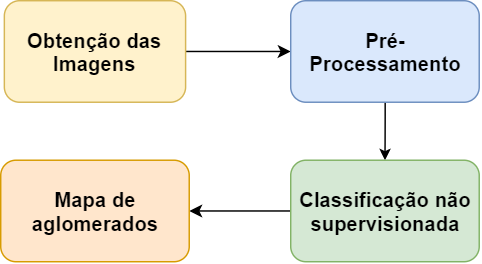
\includegraphics[width=0.55\textwidth]{images/metodo.png}
    \caption{Fases de desenvolvimento}
    \label{fig:metodo}
\end{figure}

\section{Obtenção das Imagens}

Uma vez que o projeto almeja analisar grandes quantidades de imagens de moda e suas características, foi buscado um conjunto de imagens para que fosse utilizado durante todo o processo e qualificado para treinamento e teste do modelo como um todo. Esta busca portanto seguiu duas premissas básicas: Ter disponibilidade livre de custos e ser relacionado a moda. 

Os estudos relacionados mencionados ou utilizam um dataset próprio ou buscam algum já com algum tipo de segmentação pré-aplicada para servir de base e crescer em cima dele. A obtenção das imagens de muitos destes se faz através das redes sociais, partindo do principio que estas estão disponíveis para uso público, para aplicar alguma segmentação ou fazer análises diversas. Porém, devido ao escopo deste projeto e a árdua tarefa manual de construir esta estrutura, não se faz possível coletar uma coleção de imagens próprias e realizar sua segmentação. Assim, para que o trabalho mantivesse seu foco na análise das imagens em si, houve necessidade de utilização de um dataset pronto. 

O único conjunto de dados de conhecimento voltado para moda ("Runway2Realway dataset") não é público para análise e o "DeepFashion", com a maior quantidade de imagens anotadas até o momento, requer um contato direto para solicitação de acesso. Portanto, seguindo as premissas e limitações mencionadas, a busca resumiu-se ao dataset "ModaNet" ("DeepFashion2" não havia sido disponibilizado até então). 

Este, já discutido, é um banco de anotações livre para estudos de visão computacional, disponível online e construído em cima do "Paper doll" \cite{paperdoll}. O "Paper doll", por sua vez, contém 1.097.474 de imagens coletadas de uma rede social denominada "Chictopia", voltada para que seus usuários divulguem fotos de suas roupas, construindo uma rede de criadores de estilo. As fotos têm como características principais pessoas em cenários do cotidiano, de corpo inteiro, em poses diversas, dando enfoque a suas vestimentas, como ilustra a Figura \ref{fig:paperdoll-modanet}. 

\begin{figure}
\centering
  \begin{subfigure}[b]{0.2\textwidth}
  \centering
    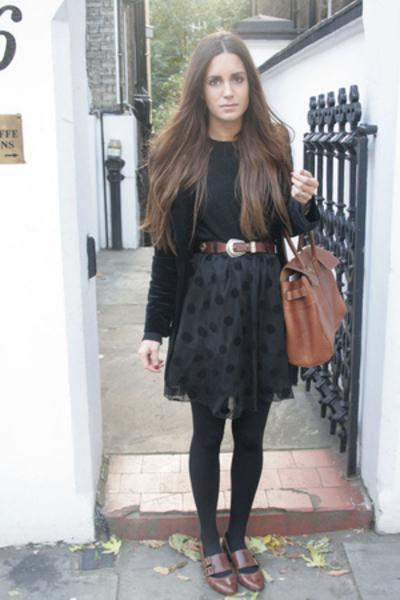
\includegraphics[scale=0.2]{images/paper1.jpg}
  \end{subfigure}
  %
  \begin{subfigure}[b]{0.2\textwidth}
  \centering
    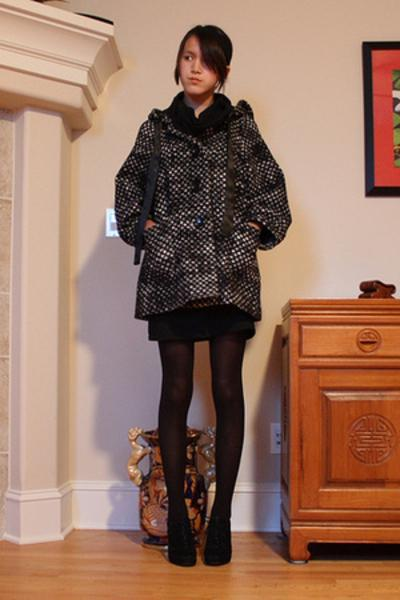
\includegraphics[scale=0.2]{images/paper2.jpg}
  \end{subfigure}
  
  \begin{subfigure}[b]{0.2\textwidth}
  \centering
    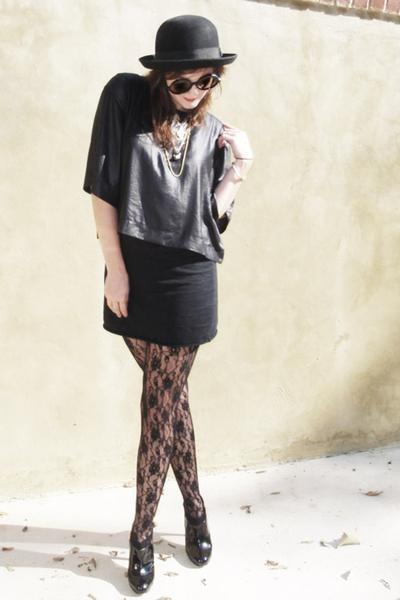
\includegraphics[scale=0.2]{images/paper3.jpg}
  \end{subfigure}
  %
  \begin{subfigure}[b]{0.2\textwidth}
  \centering
    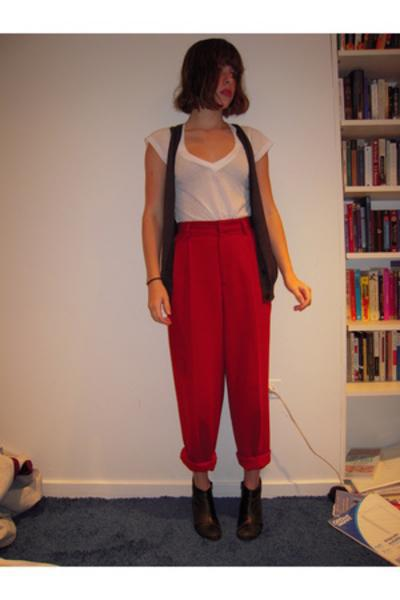
\includegraphics[scale=0.2]{images/paper4.jpg}
  \end{subfigure}
  \caption{Exemplo de imagens selecionadas pelo "ModaNet" para anotação}
  \label{fig:paperdoll-modanet}
\end{figure}

O "ModaNet" \cite{modanet} coletou dentre as milhares de imagens as com melhor resolução, exposição de vestimentas, garantindo ainda variação de poses e diversificação das classes adotadas. Assim, este é composto por anotações de 55.176 imagens no total, 52.377 de imagens para treinamento e as 2.799 restantes para validação, inteiramente anotadas em formato JSON como ilustrado na Figura \ref{fig:JSONformat}. Com informações diversas sobre a imagem, como por exemplo: tamanho da imagem, nome, identificador único no banco de imagens do "Paper doll", ainda conta com anotações dos tipos polígono e caixas delimitadoras.

\begin{figure}
    \centering
    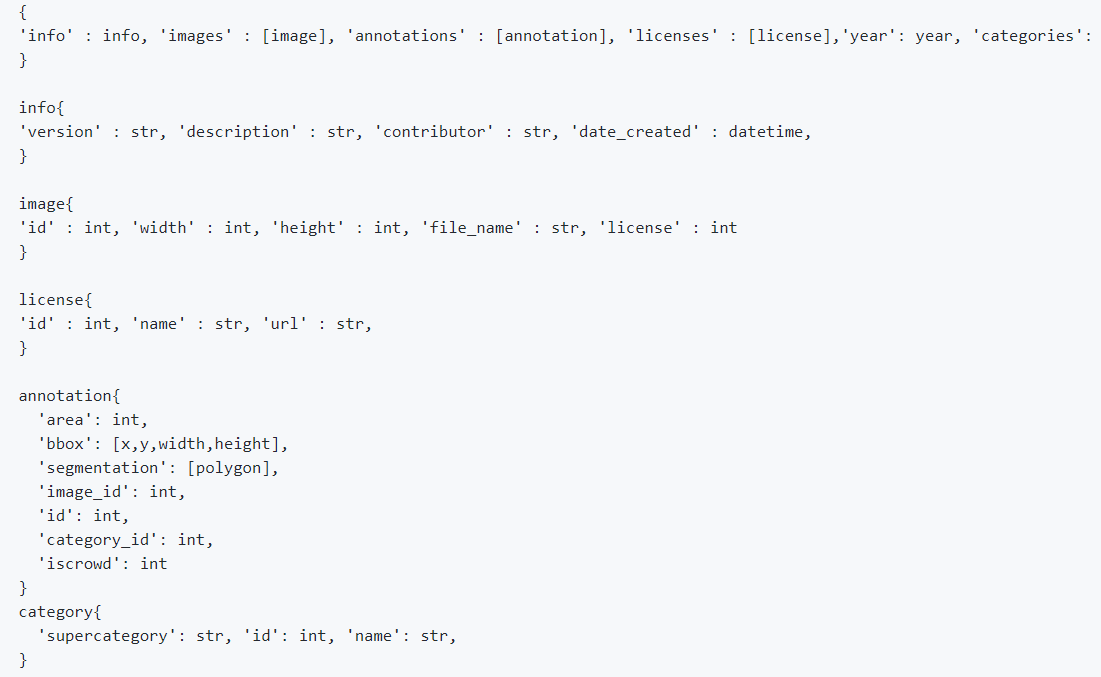
\includegraphics[width=\textwidth]{images/JSONformat.png}
    \captionsource{Formato JSON de anotação das imagens do banco de anotações "ModaNet".}{ \protect\cite{modanetgit}}
    \label{fig:JSONformat}
\end{figure}

Entretanto, dentre o total de anotações do "ModaNet", apenas as de treinamento são disponibilizadas para uso público, sendo as de validação incentivadas para que os pesquisadores submetam suas anotações como forma de desafio. Sendo assim, para este trabalho foram adotadas somente as 52.377 imagens já anotadas e feito destas os três conjuntos de anotações necessários para aplicar na rede neural: O de treinamento, com 80\% do total e validação e teste com 10\% cada. 

Com as anotações divididas em três, obteve-se acesso ao banco de imagens do "Paper doll" e, através da sua ferramenta disponibilizada como suporte para acesso a seu banco de imagens, salvou-se apenas as que haviam anotações para os identificadores únicos correspondentes. No fim, aplicando a porcentagem pré-determinada de separação das anotações, foram obtidas 41.902 imagens para treinamento, 5237 para validação e 5238 para teste, todas com resolução 600x400 pixels.

\section{Pré-Processamento}

O pré-processamento necessário para as imagens obtidas se faz necessário para minimizar o ruído na análise decorrente do fundo das imagens, isto é, o que não contém roupas. Nesta etapa foram adotadas duas metodologias aplicando a mesma rede neural de segmentação: segmentar a pessoa presente na imagem, assim como segmentar peças de roupa presentes na imagem. Dessa forma o sistema obtém visão voltada para o uso sobre a moda, ao invés de analisar imagens por completo. 
Para a realização da segmentação das pessoas e das instâncias contidas em cada imagem obtida foi aplicado uma implementação de rede neural do tipo \textit{Mask} R-CNN especialista em detecção de objetos e segmentação. Esta \cite{maskrcnnimplem}, serve como uma estrutura pronta para aplicações de detecções utilizando imagens ou vídeos, sendo já preparada para receber anotações a nível de pixel de diferentes contextos, assim como as classes correspondentes a cada anotação de roupa.

\subsection{Modelagem das Anotações}

A utilização da \textit{Mask} R-CNN como uma estrutura pronta ajuda na abstração do funcionamento de todas as etapas, sendo necessário configurar e executar somente partes interessadas ao projeto. Do código disponibilizado \cite{maskrcnnimplem}, a adaptação para novos domínios de aprendizado se faz configurando poucas funções, majoritariamente as funções de carregar as imagens e as devidas suas anotações. Entretanto para vinculação desta rede neural da com o banco de anotações "ModaNet", se faz necessário modificação do formato de anotações fornecido para deixar no formato padrão de anotações da rede.

Como ilustra a Figura \ref{fig:json-modanet}, o objeto "anotação" do arquivo JSON possui uma chave contendo um identificador único da imagem (image\_id), assim como suas instâncias descritas por polígonos, a categoria (category\_id) da instância correspondente, etc. Na figura uma forma de anotação possível do modanet para uma instância é ilustrada, a chave "segmentation" corresponde a quais pixels pertencem ao item de class "category\_id" de uma imagem identificada por "image\_id". Como cada vetor simboliza um polígono delimitador de pixels para uma peça de roupa, em casos de plural, como no exemplo acima, a instância precisa ser descrita por polígonos separados. Este caso ocorre por diferentes motivos, seja devido a sobreposição de roupa cobrir partes da instância ou devido a limitação 2d da figura.

\begin{figure}
    \centering
    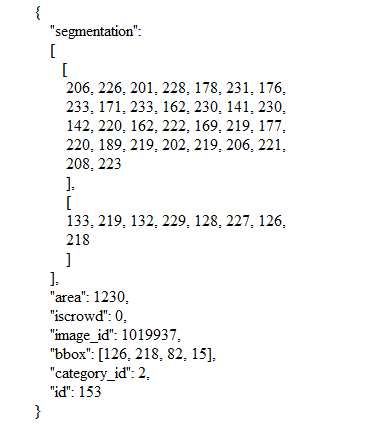
\includegraphics[scale=0.8]{images/json-modanet.png}
    \caption{Exemplo de uma anotação do "ModaNet" para a instância "cinto" na imagem 1019937}
    \label{fig:json-modanet}
\end{figure}

Os vetores de segmentação são caracterizados sempre por um valor par de pixels, iniciando com um valor na coordenada X, seguido por um valor Y, até o fim. Ainda, a estrutura da Figura \ref{fig:json-modanet} repete-se no banco de anotações para cada nova instância de uma imagem. Para uma imagem contendo, por exemplo, camiseta, calça, bolsa e sapatos anotados, essa estrutura se repetirá para cada uma destas e duas vezes para os sapatos, anotados sempre separados. 

Portanto, devido a esta falta de padronização nas anotações de haver várias segmentações separadas para uma mesma imagem, assim como um mesmo vetor conter coordenadas para X e Y, como ainda uma mesma instância ter múltiplos vetores, se fez necessário adaptar as anotações para o padrão da rede neural utilizada. 

A rede \textit{Mask} R-CNN segue um padrão para construção do seu banco de imagens interno utilizado para treinamento da rede, sendo composto da vinculação de imagens com suas anotações e classes correspondentes. A adição de imagem nesse banco espera receber cada imagem descrita pelo conjunto de classes que ela pertence, um número único, o caminho para o arquivo físico, o tamanho em largura e altura, todos o polígonos e a lista de classes disponíveis. A parte responsável por desenhar os polígonos nas imagens, por sua vez, segue o padrão de receber os polígonos das coordenadas X separadamente dos polígonos para as coordenadas Y, ambos em formato de vetores de coordenadas. 

Dessa forma, para adicionar as imagens ao modelo, foi criado então um verificador de quantas segmentações há para cada imagem única e estas salvas de forma unificada para que fossem passadas todas de uma vez só para cada imagem adicionada. Sendo necessário também após adicionar as imagens criar um verificador para separar todas as segmentações em vetores só com coordenadas X e só com coordenadas Y, para que as instâncias pudessem ser desenhadas propriamente pelo modelo. 

\subsection{Segmentação de Roupas e de Pessoas}

Nesta etapa do pré-processamento a rede neural é utilizada para segmentar roupas e pessoas. A obtenção do banco de imagens "ModaNet" compõe parte da primeira segmentação, onde a rede é exposta a milhares de imagens contendo diferentes tipos de roupas para aprender a encontrá-las em novas imagens. A segunda segmentação, por sua vez, se torna mais simples devido a redes pré-treinadas para detecção de objetos do cotidiano, incluindo pessoas. 

A \textit{Mask} R-CNN, devido sua estrutura pronta para uso, fornece apoio para treinamento com pesos pré-treinados a fim de agilizar o treinamento em novos domínios. O treinamento de redes neurais complexas como esta partindo do início podem demorar dias, exigir muito recurso computacional, assim como o processo de tunar seus parâmetros ou melhorar sua performance podem ser muito desafiadores. Portanto, \cite{maskrcnnimplem} fornece as opções de treinar a rede utilizando os pesos --- valores que definem o aprendizado da rede --- de redes já treinadas em domínios genéricos, como também treinar a rede do início partindo de pesos aleatórios. Dessa forma, as duas segmentações realizadas seguiram métodos diferentes, devido a origem de cada problema. 

Devido a não existência de redes pré-treinadas e disponíveis sob o domínio de roupas, se faz necessário retreinar a rede sob este domínio. O treinamento para segmentação de roupas foi realizado, portanto, sobre os pesos pré-treinados da rede para o domínio "COCO" (Objetos Comuns em contexto, do inglês, \textit{Common Objects in Context}) \cite{COCO}, enquanto que para segmentação de pessoas foram utilizados os mesmos pesos, porém agora sem precisar retreinamento já que a classe "pessoa" já faz parte do treinamento original.

"COCO", assim como "ImageNet" (Desafio de Reconhecimento Visual em Larga Escala ImageNet, do inglês \textit{ImageNet Large Scale Visual Recognition Challenge} - ILSVRC) \cite{imagenet}, são banco de imagens construídas por organizações com intuito de propor desafios de detecção, classificação e reconhecimento de cenas de forma geral na área de visão computacional. Tendo 91 e 1000 objetos do cotidiano, respectivamente, em sua abrangência, estes bancos buscam generalizar a visão computacional e portanto contribuem com o avanço do estudo na área por servirem de treinamento para redes neurais diversas, posteriormente disponibilizadas online. A utilização de pesos destas redes para treinar a rede em outro domínio, diferentemente de transferência de aprendizado, serve como impulso para chegar a outro aprendizado mais simples, uma vez que o domínio mais complexo já aprendeu muitos padrões e regras que provavelmente seriam aprendidos pelo outro domínio mais simples.

Para o treinamento utilizando as anotações de roupas o modelo não demora a baixar sua função custo para um valor menor que 2, porém houve dificuldade em fazer o modelo reduzir de 1, obtendo-se em melhores experimentos em torno de 1,4. Foram variadas as configurações de épocas, validação por época e passos por época, porém para os testes e dados fornecidos o modelo se mostrou resistente a chegar numa função custo próxima de zero mostrando a partir desse ponto limitação na capacidade de aprendizado. 

\section{Classificação Não Supervisionada de Aglomerados}

Após a obtenção e pré-processamento das imagens concluídos, estas podem finalmente ser utilizadas para classificação não supervisionada em forma de aglomerados. Para isso foi adotado uma sequência de passos consistindo da extração de características das imagem, redução da dimensão destas características, aplicação do \ac{t-SNE} e por fim a construção do mapa bi-dimensional desejado. Este algoritmo seguido para extração de característica e aplicado como transferência de aprendizado tem se provado eficiente e usado para fins didáticos, neste trabalho tendo sido feito uma adaptação da implementação disponibilizada pelo Gene Kogan \cite{ml4a}, cientista que impulsiona o ensino de visão computacional para artistas de forma gratuita.

\subsection{Extração de Características}

Para a extração de características se faz necessário uma rede treinada em domínio genérico de forma a simular uma visão geral do mundo e fornecer uma abstração de características gerais presentes em uma imagem. Se houvessem redes treinadas no domínio de roupas seria ideal, porém como não há, opções viáveis se voltam a modelos pré-treinados e renomados por desafios de visão computacional de domínios genéricos.  Para a tarefa de classificação de imagens o desafio já citado "ImageNet" é considerado referência \cite{pyimage} e tem sido dominado por redes neurais convolucionais e diferentes técnicas de aprendizado profundo desde 2012. Assim sendo, na biblioteca utilizada para implementação são disponibilizadas algumas das redes neurais já treinadas que apresentaram melhor desempenho no desafio durante os anos, prometendo forte habilidade de generalização para aplicações com imagens fora do domínio do "ImageNet".

Dentre as redes disponibilizadas pelo Keras se encontram "VGG16", "VGG19", "Xception", "Resnet" e "InceptionV3", para nomear as mais famosas. A aplicação de qualquer destes modelos pode ser feita para extração de características das imagens, esperando idealmente obter com qualquer destes modelo alta performance na obtenção de descritores. Devido terem sido treinados sob o mesmo número de imagens e sob as mesmas classes de classificação, induzindo terem os mesmos \textit{kernels} de convolução, o modelo pré-treinado escolhido para aplicar no projeto focou em um considerado leve \cite{pyimage}, a terceira versão da rede do projeto "Inception" da Google, "InceptionV3". 

Sendo a versão mais recente disponível na biblioteca Keras dos modelos "Inception", esta versão apresenta baixo custo computacional se comparado a suas alternativas, tendo atingido 17,2\% de erro top-1 na ILSVRC de 2012 \cite{inceptionv3}. Sua arquitetura, ilustrada na Figura \ref{fig:inceptionv3}, consiste dentre outras de uma grande quantidade de operações de convolução feitas em paralelo para otimizar o processo. Como seu uso aqui se faz para extração de características, é preciso utilizar a arquitetura ignorando suas últimas camadas responsáveis pela classificação das classes do ImageNet ("Fully Connected" e "softmax" na Figura \ref{fig:inceptionv3}), resultando em vetor de características multidimensional de tamanho 1x2048.

%obtendo-se assim um vetor que descreve a imagem de entrada em sua menor dimensão. Para a VGG-16, ilustrada na figura \ref{fig:vgg16}, o modelo deve ser limitado a camada "fully connected + ReLU" com saída de tamanho 1x4096, ou seja, um vetor contendo 4096 valores descritivos da imagem.

%destacas só a, VGG-16, deriva do projeto VGG da universidade de Oxford [ref] para investigar como a profundidade das redes convolucionais afetam sua acurácia em um sistema de reconhecimento em larga escala. Conseguindo 71,5\% de acurácia no ILSRC de 2012, o modelo apresenta grande capacidade de generalização, chegando a 91,8\% no banco de imagens Caltech-101. Inception V3, do projeto Inception da Google, apresenta uma rede muito mais complexa que a VGG-16, conseguindo atingir 78.2\% de acurácia no ImageNet em 2015, porém com uma redução de 36 vezes na quantidade de parâmetros se comparada com a VGG-16. 

\begin{figure}
    \centering
    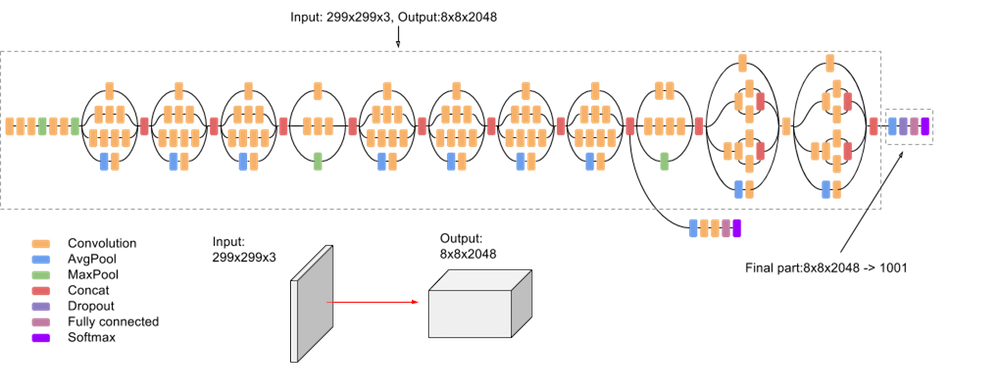
\includegraphics[scale=0.5]{images/inceptionv3.png}
    \captionsource{Arquitetura do modelo InceptionV3.}{ \protect\cite{inceptionarch}}
    \label{fig:inceptionv3}
\end{figure}

%Nas arquiteturas \ref{fig:vgg16} e \ref{fig:inceptionv3} também pode ser notado que o tamanho das imagens de entrada nas redes são de baixa qualidade: VGG-16 funciona com imagens coloridas de tamanho 224x224, 

Ainda, outro ponto importante é o tamanho das imagens aceitas por estes tipos de redes. Todas os modelos de redes mencionados possuem uma limitação inerente ao desafio do "ImageNet", devido a grande quantidade de classe que as redes precisam aprender e ao grande número de parâmetros para serem treinados. Portanto, a "InceptionV3"  aceita imagens de tamanho exclusivo 299x299, levando a necessidade de redimensionar para este tamanho todas as imagens que serão utilizadas.

\subsection{Redução da Dimensionalidade e Visualização de Aglomerados}

São obtidos milhares de valores para as características de cada imagem, dificultando o entendimento e organização desses dados. Para conseguir uma redução ainda maior de dimensão dos descritores do que a já feita pelas camadas da rede de extração, optou-se por realizar redução dimensional através de Análise de Componentes Principais.

A aplicação de um redutor de dimensionalidade ajuda na síntese dos dados não só na eficiência em tratar menos dados, como também evitando redundância de características. Operar sobre 2048 elementos para cada imagem, por exemplo, é ineficiente em termos de processamento e convergência, logo se estes mesmos dados podem ser representados através de menos dados de forma a não perderem o significado, a performance como um todo é melhorada. Na sua redução \ac{PCA} não só mantém uma representação razoável aos dados originais, como também evita a redundância de informações para que manter apenas as singulares.

A aplicação do \ac{PCA} utilizada segue a implementação da biblioteca "scikit-learn" \cite{sklearnPCA} baseada nas implementações de LAPACK \cite{LAPACK} e \cite{truncated}, completa ou truncada dependendo do tamanho dos dados de entrada e do número de componentes para extrair. Devido a abstração da biblioteca, o uso desta ferramenta \ac{PCA} requer atenção apenas na regularização dos parâmetros "número de componentes principais" e "tipo de solucionador". 

O número de componentes corresponde a quantidade de componentes para serem mantidos de acordo com a porcentagem de informação relevante mantida pelos eixos. A única limitação da escolha deste valor é o valor mínimo entre o número de amostras de imagens e o número de características obtidas. O número de PC's pode ser determinado manualmente, de forma arbitrária, ou ser determinado pelo algoritmo de Minka \cite{minka} para detecção automática de dimensões. O solucionador é escolhido automaticamente pela biblioteca a depender do tamanho dos dados de entrada, podendo ser também alterado para versões truncadas ou completas dos algoritmos existentes para PCA \cite{sklearnPCA}.

Após a aplicação do PCA, as dimensões devem ser reduzidas de milhares para a escala de dezenas ou centenas, neste ponto os dados se encontram em um espaço intermediário onde sua redundância foi reduzida. Os mapas de características fornecidos pela rede devem apresentar valores semelhantes para imagens semelhantes, mostrando coerência de entendimento das imagens. Logo, para analisar a semelhança desses vetores de características é aplicado a distância do cosseno, implementada também pelo "scikit-learn", onde esta recebe dois vetores e retorna uma medida de dissimilaridade entre estes. Neste ponto grandes análises podem ser feitas, como por exemplo, achar imagens entendidas como semelhantes pelo extractor de imagens, verificar assim a acurácia dos mapas de características e ainda da redução de dimensionalidade.

Muito embora imagens semelhantes já possam ser visualizadas neste ponto através da distância do cosseno, a ideia é trazer as imagens para 2-d onde poderão ser vistas e comparadas como um todo. Portanto, \ac{t-SNE} pode ser aplicado como outra ferramenta para redução das dimensões dos dados e possibilitar a visualização destes em 2 ou 3 dimensões. Esta ferramenta, que converte similaridade entre pontos para probabilidade conjunta e tenta minimizar a divergência de "Kullback-Leibler" entre as probabilidades conjuntas nos espaços de alta e baixa dimensão simultaneamente, tem por definição uma função custo não conexa, fazendo com que diferentes inicializações e parâmetros resultem em diferentes resultados de visualizações --- ainda que coerentes. Sua aplicação é altamente recomendada a ser utilizada em conjunto com outro métodos de redução de dimensão para dados esparsos, levando os dados de uma alta quantidade de dimensões para um espaço intermediário. Este processo não só agiliza o processamento do algoritmo, como também evita ruídos melhorando a acurácia das novas representações \cite{sklearntSNE}. 

A implementação do \ac{t-SNE} utilizada também baseou-se na disponibilizada pela biblioteca "scikit-learn", tendo alguns parâmetros do processo de otimização para regular na sua execução, estes responsáveis por muitas vezes gerar diferentes imagens de resultados: Número de componentes, perplexidade, taxa de aprendizado e ângulo. O número de componentes aqui é equivalente ao do PCA, sendo um valor inteiro para a quantidade de dimensões que o algoritmo deve reduzir os dados (mantido em 2 nesta aplicação); A perplexidade refere-se ao número de aglomerados independentes que o \ac{t-SNE} vai tentar classificar os dados, orientado pelo artigo original \cite{tsnepaper} para estar entre 5-50; A taxa de aprendizado (10-1000) equivale a um valor numérico que orienta na convergência do algoritmo, alterações neste valor implicam diretamente na visualização final. Foi mantido um valor alto de por volta dos 200, pois valores muitos altos forçam o mapa a parecer com uma bola e o valor escolhido mostrou bons espalhamentos; Por fim, o ângulo controla a troca de custo entre velocidade e acurácia, para valores baixos a acurácia promete ser melhor, porém demora mais tempo para processar --- foi utilizado um valor de 0.2 para todos os teste.  

Uma vez configurado todos os parâmetros do \ac{PCA} e do \ac{t-SNE}, as imagens podem finalmente serem representadas no espaço bidimensional aglomeradas com suas semelhantes. Em teoria o algoritmo do \ac{t-SNE} aceita qualquer quantidade de imagens e pode gerar um resultado visual com grande quantidade de aglomerados. Devido a tantas variáveis e a subjetividade da visualização, as técnicas foram aplicadas repetidas vezes, sob diferentes configurações.

Por fim, para dar outra forma de visibilidade e sem sobreposição de imagens, como no formato em aglomerados, é aplicado uma ferramenta de transformação de mapas \ac{t-SNE} em formato de grid. Para isto foi aplicada a versão nativa do Python disponibilizada com nome "RasterFairy", adaptada da versão disponibilizada do \cite{kogan}, voltada para transformar qualquer nuvem de pontos (neste caso imagens) em uma estrutura regular de tabela, enquanto preservando as relações de vizinhança. Mario Klingemann \cite{raster} ilustra esta transformação de estruturas de forma intuitiva utilizando uma animação, exemplificada na Figura \ref{fig:raster}. 

\begin{figure}
  \centering
  \begin{subfigure}[b]{0.4\textwidth}
  \centering
    \includegraphics[width=\textwidth]{images/raster1.png}
    %\caption{}
    \label{fig:mask1}
  \end{subfigure}
  %
  \centering
  \begin{subfigure}[b]{0.4\textwidth}
  \centering
    \includegraphics[width=\textwidth]{images/raster2.png}
    %\caption{}
    \label{fig:mask3}
  \end{subfigure}
  %
  \captionsource{Ilustração do funcionamento do "RasterFairy". }{ \protect\cite{raster}}
  \label{fig:raster}
\end{figure}


\chapter{Resultados}
\label{cha:resultados}

Os resultados deste trabalho devem ser descritos por toda sua cadeia de desenvolvimento, muito embora seu resultado final seja claro quanto mapa que deseja-se obter. As imagens utilizadas para ilustração dos resultados são as mesmas anotadas pelo "ModaNet", todas compostas por apenas uma pessoa em cena, em cenário cotidiano e de tamanho padrão 600x400 pixels de resolução.  

\section{Segmentações}

\subsection{Segmentação de Vestimentas}

Como mencionado, antes de treinar a rede neural para aprender a segmentar instâncias de vestimentas foi modelado o banco de anotações para se adequar a sintaxe exigida pela \textit{Mask} R-CNN utilizada. O resultado desta alteração, ilustrado na Figura \ref{fig:masks}, mostra como a rede passou a entender as anotações a nível de pixel, após a modelagem aplicada. O exemplo ilustrado selecionou 3 imagens aleatórias do subconjunto de treinamento.

\begin{figure}
  \centering
  \begin{subfigure}[b]{\textwidth}
  \centering
    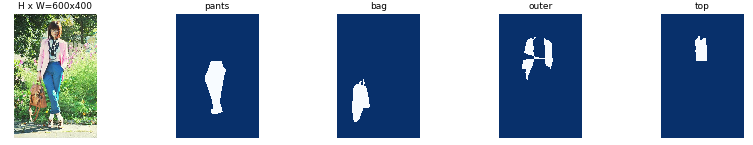
\includegraphics[scale=0.8]{images/mask1.png}
    %\caption{}
    \label{fig:mask1}
  \end{subfigure}
  %
  \centering
  \begin{subfigure}[b]{\textwidth}
  \centering
    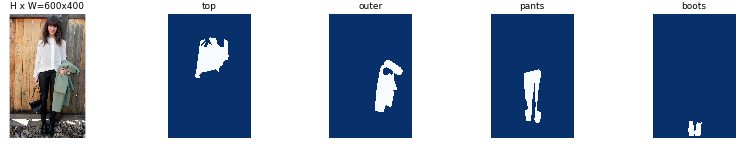
\includegraphics[scale=0.8]{images/mask3.png}
    %\caption{}
    \label{fig:mask3}
  \end{subfigure}
  %
  \centering
  \begin{subfigure}[b]{\textwidth}
  \centering
    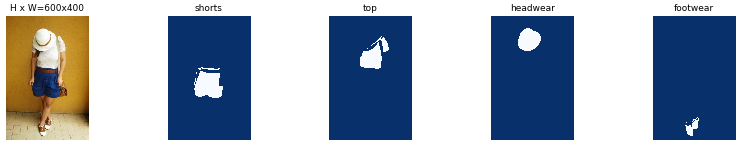
\includegraphics[scale=0.8]{images/mask2.png}
    %yo\caption{}
    \label{fig:mask2}
  \end{subfigure}
  \caption{Inspeção do funcionamento da modelagem de anotações no padrão da rede neural utilizada. As classes ilustradas são respectivamente: Calça, bolsa, sobretudo, blusa, sapatos, shorts e chapéu.}
  \label{fig:masks}
\end{figure}
 
O resultado da segmentação se mostrou satisfatório para muitos casos, conseguindo detectar muitas instâncias diferentes de roupas em imagens com diferentes padrões de exposição e poses. Entretanto, devido a grande quantidade de poses e estilos de roupas presentes nas imagens, muitos exemplos de detecção falham em detectar a roupa por completo ou a instância toda. Foi percebido que a instância calça é muitas vezes entendida como presente na imagem, mesmo sem estar presente e a instância bolsa e sapatos se mostram as com melhores resultados, talvez devido estarem menos expostas a ruídos de braço, assim como misturas e peças de roupas. Algumas instâncias se mostraram pouco reconhecidas, como óculos, bota, sobretudo e jaqueta, enquanto que outras mostraram pouca capacidade de entender a roupa por completo, como blusa que muitas vezes gera uma instância parcial da blusa. 

Na Figura \ref{fig:moda-seg}, podemos ver um exemplo onde as instâncias são detectadas com êxito podendo serem separadas da imagem sem perder seu valor para outros usos. Enquanto que na Figura \ref{fig:moda-seg2}, por sua vez, é apresentado um caso onde a bolsa e os sapatos são detectados, porém o vestido é interpretado como vestido, saia e blusa ao mesmo tempo, tendo ainda sido reconhecida uma calça inexistente. 

\begin{figure}
  \centering
  \begin{minipage}[b]{0.3\textwidth}
    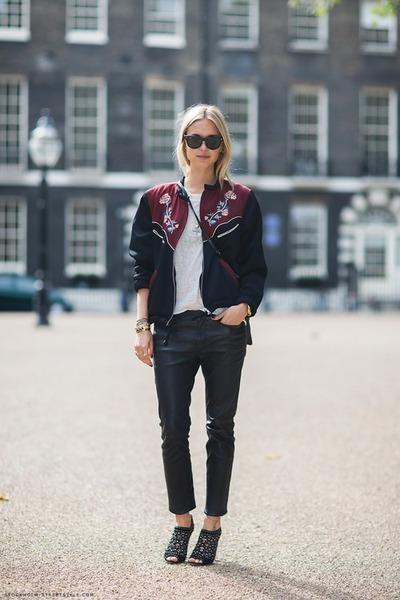
\includegraphics[width=\textwidth]{images/resultados/1060077original.jpg}
  \end{minipage}
  \hfill
  \begin{minipage}[b]{0.3\textwidth}
    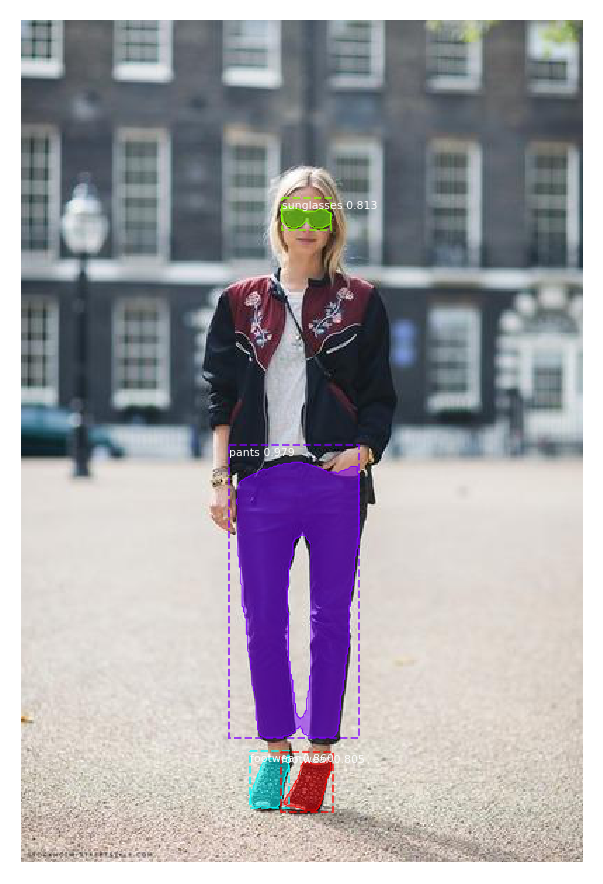
\includegraphics[width=\textwidth]{images/resultados/1060077roupas.png}
  \end{minipage}
    \hfill
  \begin{minipage}[b]{0.3\textwidth}
    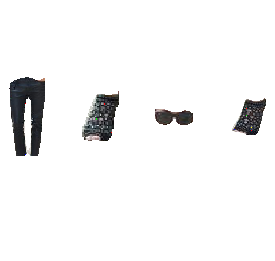
\includegraphics[width=\textwidth]{images/resultados/1.png}
  \end{minipage}
  \caption{Resultados de segmentação de vestimentas implementado.}
  \label{fig:moda-seg}
\end{figure}

\begin{figure}
  \centering
  \begin{minipage}[b]{0.48\textwidth}
    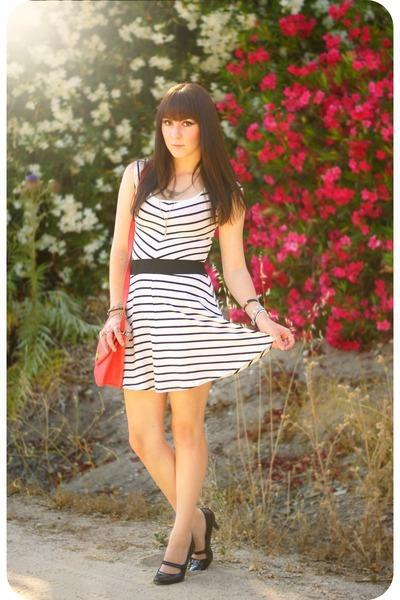
\includegraphics[width=0.8\textwidth]{images/resultados/490842original.jpg}
  \end{minipage}
  \hfill
  \begin{minipage}[b]{0.48\textwidth}
    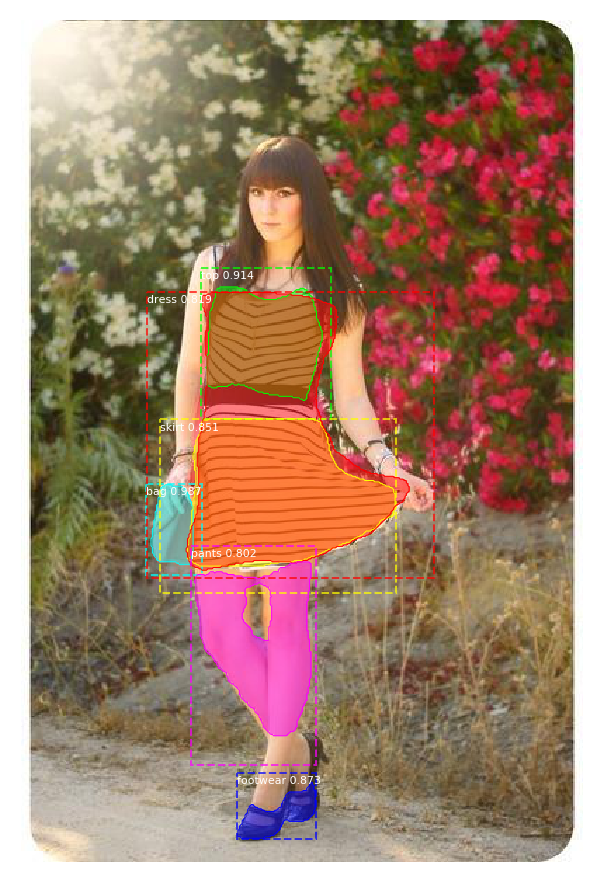
\includegraphics[width=0.8\textwidth]{images/resultados/490842roupas.png}
  \end{minipage}
    \hfill
  \begin{minipage}[b]{0.7\textwidth}
    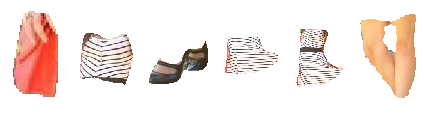
\includegraphics[width=\textwidth]{images/resultados/2.png}
  \end{minipage}
  \caption{Problemas na segmentação de vestimentas, classe errada e instância inexistente.}
  \label{fig:moda-seg2}
\end{figure}

Neste ponto se fez difícil analisar a capacidade da rede de segmentação de vestimentas de forma precisa, não conseguindo chegar a uma conclusão precisa ou aplicada uma metodologia já utilizada para medir a capacidade de segmentação da rede treinada sobre as imagens de teste. 

\subsection{Segmentação de Pessoas}

A segmentação de pessoas foi aplicada também as imagens do "Paperdoll" obtidas, porém executada na rede sobre os pesos pré-treinados para as classes do cotidiano COCO, que dentre as 80 classes possíveis limitou-se a reconhecer somente a classe "Pessoa". Este processo de reconhecimento da instância "pessoa" possibilitou a criação de novas imagens contendo somente a instância detectada na imagem original, como ilustrado na Figura \ref{fig:person-seg}. 

\begin{figure}
  \centering
  \begin{minipage}[b]{0.3\textwidth}
    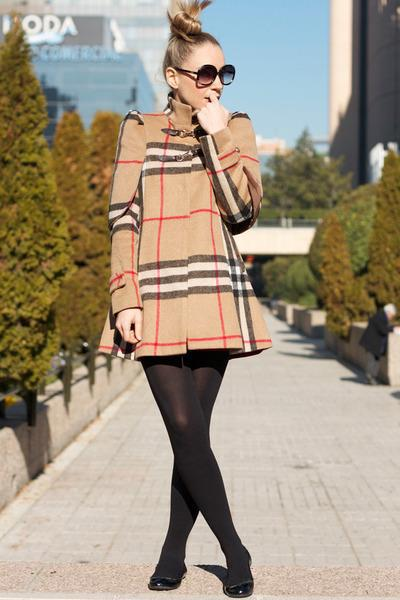
\includegraphics[width=\textwidth]{images/resultados/299206original.jpg}
    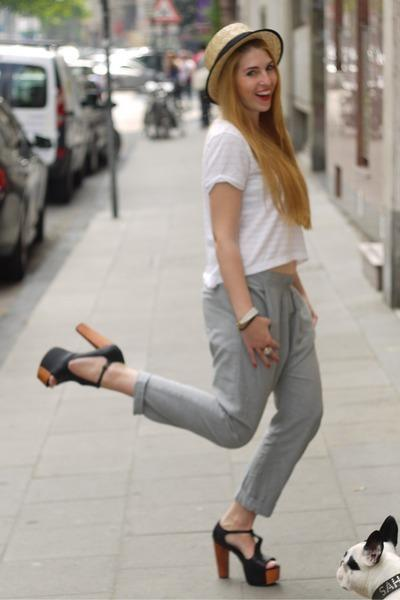
\includegraphics[width=\textwidth]{images/resultados/349322original.jpg}
    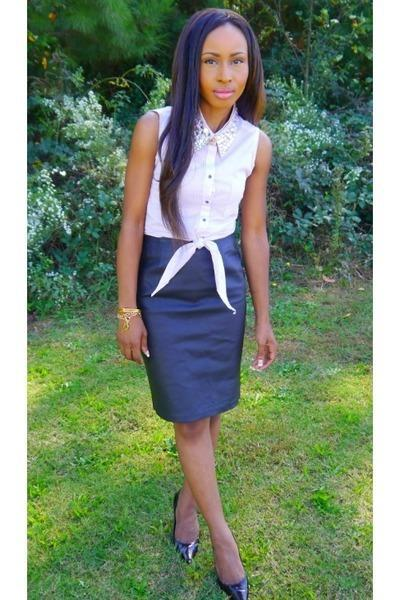
\includegraphics[width=\textwidth]{images/resultados/1082993original.jpg}
  \end{minipage}
  \hfill
  \begin{minipage}[b]{0.3\textwidth}
    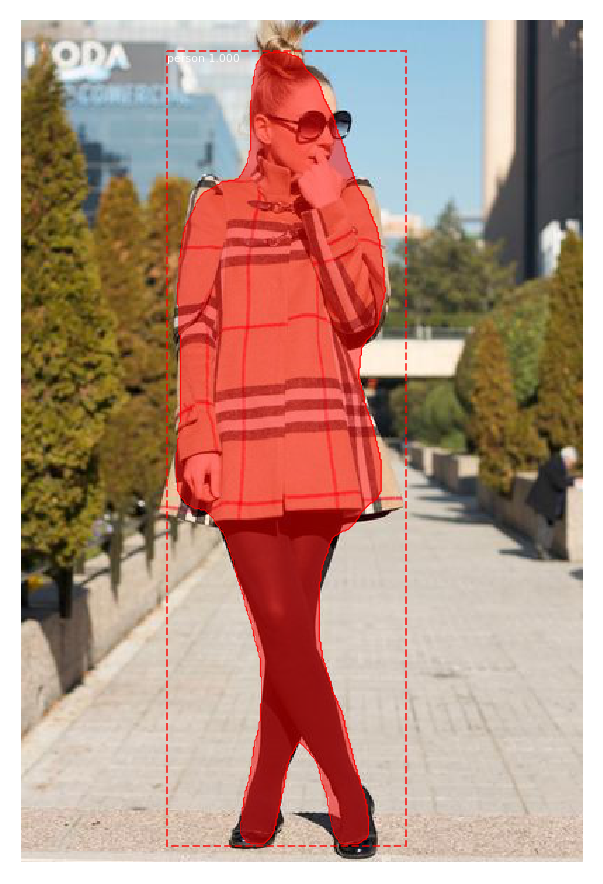
\includegraphics[width=\textwidth]{images/resultados/299206person.png}
    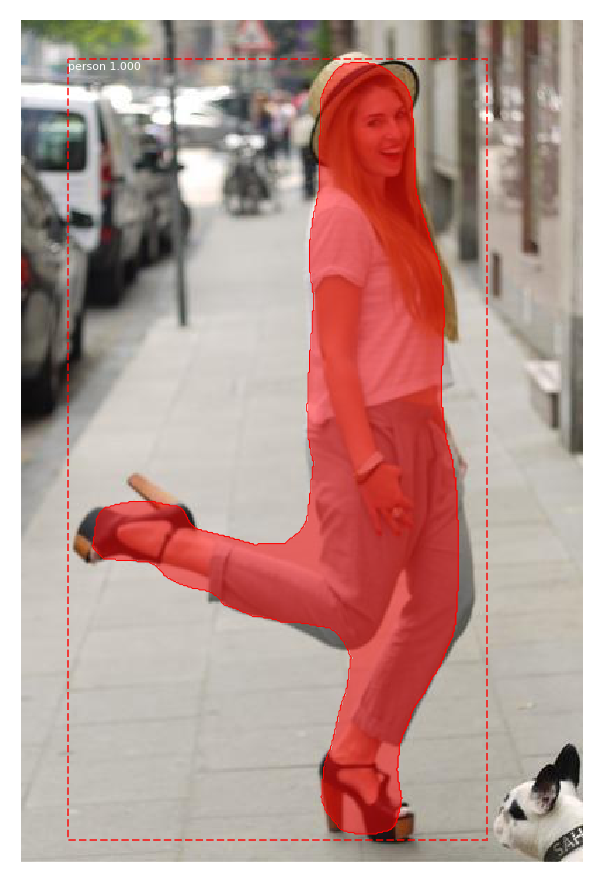
\includegraphics[width=\textwidth]{images/resultados/349322person.png}
    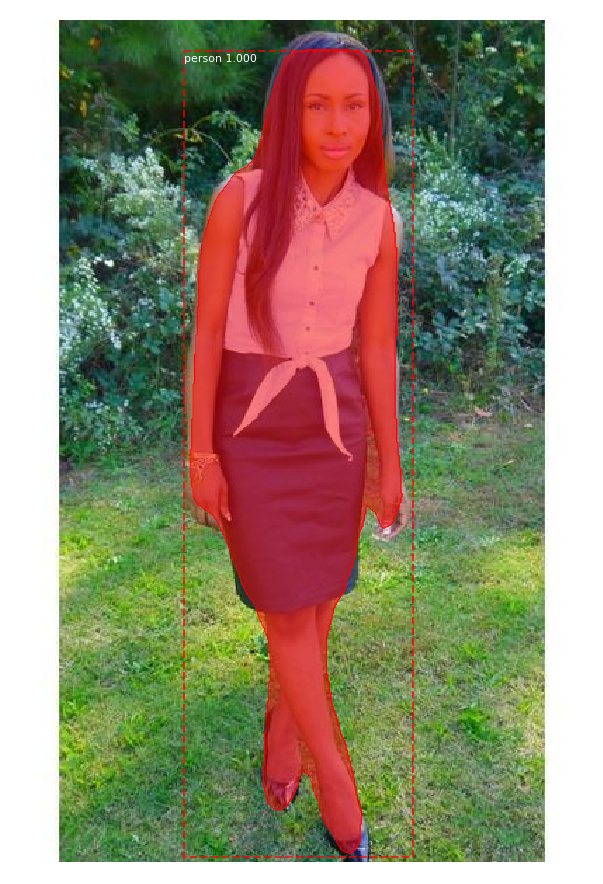
\includegraphics[width=\textwidth]{images/resultados/1082993person.png}
  \end{minipage}
    \hfill
  \begin{minipage}[b]{0.3\textwidth}
    \includegraphics[scale=0.5]{images/resultados/299206mask.jpg}
    \includegraphics[scale=0.5]{images/resultados/349322mask.jpg}
    \includegraphics[scale=0.5]{images/resultados/1082993mask.jpg}
  \end{minipage}
    \hfill
  \caption{Resultados de segmentação de pessoas implementada.}
  \label{fig:person-seg}
\end{figure}

Os resultados das detecções de pessoa conseguem 100\% de acurácia para todas as detecções propostas pelas iamgens do "paper doll", porém para uma possível criação de banco de imagens a serem utilizadas para análise de moda reais a partir dos exemplos apresentados para a rede, esta não conseguiria acurácia tão alta, uma vez que a instância "pessoa" tende a seguir a forma do corpo da pessoa nas fotos utilizadas levando em alguns casos a ignorar formas de pessoas alteradas por roupas mais complexas da moda. Ainda assim, as imagens segmentadas por pessoas foram salvas e aplicadas e testadas na criação dos aglomerados para reduzir o ruído do plano de fundo. 

A grande limitação real para as imagens aplicadas nesta segmentação, entretanto, foram na geração das máscaras. Alguns exemplos se mostraram ruidosos como ilustrado na Figura \ref{fig:segsruins}, principalmente para têxturas mais complexas. Embora na maioria dos casos sejam ruídos pequenos --- os casos ilustrados mostram casos extremos --- ainda assim muitas máscaras da intância pessoa apresentam alterações nas cores de pixels pela imagem, podendo comprometer roupa. A razão desta anomalia não foi esclarecida, podendo ser um simples problema com a extensão ".png" a qual a rede utiliza para gerar as instâncias.

\begin{figure}
  \centering
  \begin{subfigure}[b]{0.4\textwidth}
  \centering
    \includegraphics[width=0.3\textwidth]{images/resultados/159.png}
    %\caption{}
    \label{fig:}
  \end{subfigure}
  %
  \centering
  \begin{subfigure}[b]{0.4\textwidth}
  \centering
    \includegraphics[width=0.3\textwidth]{images/resultados/1532.png}
    %\caption{}
    \label{fig:}
  \end{subfigure}
  \caption{Exemplos onde a segmentação de pessoa gera máscaras ruidosas.}
  \label{fig:segsruins}
\end{figure}

\section{Visualização de Aglomerados}

Os resultados dos aglomerados são ilustrados para um subconjunto de imagens escolhidas aleatoriamente dentre as imagens para os casos: Sem nenhum pré-processamento, com pessoas segmentadas e para as instâncias de roupas. 

A Figura \ref{fig:originais} ilustra como a imagem fica ao ser redimensionada para a resolução 299x299 exigida pela "Inception V3" e como se parece o vetor de características obtido na saída da rede de extração para a imagem em exemplo. Idealmente imagens similares entre si devem apresentar semelhança entre estes vetores.

\begin{figure}
  \centering
  \begin{subfigure}[b]{\textwidth}
  \centering
    \includegraphics[scale=0.7]{images/resultados/299206menor.png}
    %\caption{}
    \label{fig:}
  \end{subfigure}
  %
  \centering
  \begin{subfigure}[b]{\textwidth}
  \centering
    \includegraphics[scale=0.45]{images/resultados/299206feat.png}
    %\caption{}
    \label{fig:}
  \end{subfigure}
  \caption{Redimensionamento de imagem e seu vetor de características.}
  \label{fig:originais}
\end{figure}

Aplicando a métrica para medir distância entre os vetores, distância do cosseno, podemos comparar o vetor de características de uma imagem com de várias outras e achar os que apresentam menor distância para verificar a consistência de extração da rede. A Figura \ref{fig:compaoriginais} mostra um comparativo de imagens consideradas semelhantes por esta métrica. Ao analisar ambos os casos fica perceptível que as imagens realmente possuem semelhanças de cores, formatos e padrões em geral, muito embora sendo muito influenciadas por regiões não contendo roupa. 

\begin{figure}
  \centering
  \begin{subfigure}[b]{\textwidth}
  \centering
    \includegraphics[scale=0.45]{images/resultados/compaoriginais2.png}
    %\caption{}
    \label{fig:}
  \end{subfigure}
  %
  \centering
  \begin{subfigure}[b]{\textwidth}
  \centering
    \includegraphics[scale=0.45]{images/resultados/compaoriginais3.png}
    %\caption{}
    \label{fig:}
  \end{subfigure}
  \caption{Resultado da análise de características obtidas para imagens não segmentadas e entendidas como semelhantes.}
  \label{fig:compaoriginais}
\end{figure}

Ainda assim o t-SNE é gerado para esta coleção de imagens em duas dimensões, Figura \ref{fig:tsne1}, para um total de 200 imagens. O mapa gerado utilizou PCA para reduzir o número de características de 2048 para 50, o bastante para ser possível classificar as imagens em aglomerados. Para facilitar o entendimento visual, o mapa é colocado em formado de grid na figura \ref{fig:rast1}.

\begin{figure}
    \centering
    \includegraphics[scale=0.5]{images/resultados/tsne2.png}
    \caption{Resultado do t-SNE aplicado a imagens sem segmentação.}
    \label{fig:tsne1}
\end{figure}

\begin{figure}
    \centering
    \includegraphics[scale=0.4]{images/resultados/rast1.png}
    \caption{Resultado de grid RasterFairy aplicado a imagens sem segmentação.}
    \label{fig:rast1}
\end{figure}

Seguindo o mesmo algoritmo para as imagens de pessoas segmentadas obtém-se desta vez resultados com menor resolução, devido a natureza da criação das imagens serem imagens já serem pequenas, entretanto resultados mais relativos a vestimentas. Na Figura \ref{fig:compasegs}, fica mais claro que as imagens consideradas semelhantes agora sofrem menos ruído de outras formas que não o que as pessoas estão usando. 

\begin{figure}
    \centering
    \includegraphics[scale=0.4]{images/resultados/compasegs.png}
    \caption{Comparativo de imagens de pessoas segmentadas consideradas semelhantes.}
    \label{fig:compasegs}
\end{figure}

O mapa t-SNE obtido para um conjunto também de 200 amostras e com PCA de 50 componentes, é vista na Figura \ref{fig:tsne3} e seu respectivo grid na Figura \ref{fig:rast2}. O resultado se mostra menos confuso devido haver menos ruído nas imagens, ilustrando aglomerados de roupas semelhantes por cor e estampas. 

\begin{figure}
    \centering
    \includegraphics[scale=0.5]{images/resultados/tsne3.png}
    \caption{Resultado do t-SNE aplicado a pessoas segmentadas.}
    \label{fig:tsne3}
\end{figure}

\begin{figure}
    \centering
    \includegraphics[scale=0.4]{images/resultados/rast2.png}
    \caption{Resultado de Grid para imagens de pessoas segmentadas.}
    \label{fig:rast2}
\end{figure}

Por fim, o processo pode ser levado ao último nível de análise, quando as imagens são instâncias de roupas. Ao aplicar a extração de características sobre estas imagens, é feita uma análise somente para um tipo de roupa, por exemplo, analisar bolsa, sapatos ou vestidos. A Figura \ref{fig:compabolsa} ilustra a análise para bolsas detectadas de imagens aleatórias do banco "Paper doll", que independentemente da baixa resolução, as imagens conseguem ser associadas com suas semelhantes. O plote do t-SNE para estas intâncias não se faz interessante neste caso devido as instâncias de roupas geradas terem resolução muito baixa. 

\begin{figure}
  \centering
  \begin{subfigure}[b]{\textwidth}
  \centering
    \includegraphics[scale=0.4]{images/resultados/compabolsa.png}
    %\caption{}
    \label{fig:}
  \end{subfigure}
  %
  \centering
  \begin{subfigure}[b]{\textwidth}
  \centering
    \includegraphics[scale=0.4]{images/resultados/compabolsas2.png}
    %\caption{}
    \label{fig:}
  \end{subfigure}
  \caption{Comparativo dos descritivos obtidos para bolsas segmentadas e consideradas semelhantes.}
  \label{fig:compabolsa}
\end{figure}



\chapter{Conclusões}
\label{cha:conclusoes}

Neste trabalho foi proposto a aplicação de um algoritmo para aglomerar imagens digitais de moda de forma automática para facilitar no processo de análise destas. A principal motivação para o desenvolvimento deste trabalho é a ineficiência na absorção de coleções de moda durante a grande quantidade de coleções lançadas por ano no mundo e a quantidade de imagens distribuídas em mídias digitais destas criações. A metodologia proposta busca através de aprendizagem de máquina automatizar o entendimento destas imagens e realizar um agrupamento também automático baseado em semelhanças e diferenças. A ferramenta, que utilizou diferentes segmentações de imagens, buscou mais do que organizar imagens mas determinar características descritivas de vestimentas em geral.

As segmentações, que se dividiram em segmentação de pessoas e de instâncias, se mostraram eficientes para geração de novas imagens buscando minimizar o ruído de elementos irrelevantes das imagens. A performance da segmentação sobre o ModaNet mostrou problemático para reduzir o erro da função custo, assim como limitação na sua análise precisa de segmentação do subconjunto de imagens de teste, necessitando de um maior conhecimento da arquitetura da rede Mask para saber até onde ela conseguiria aprender sobre este novo domínio que apresenta poucos elementos de treinamento. Ainda, a "Inception V3" se mostrou eficiente na geração de características coerentes e a análise destas pela métrica utilizada mostrou uma obtenção de itens semelhantes.

Embora os resultados tenham sido ilustrados com imagens de roupas, estas em definitivo não descrevem moda, não tendo nenhuma atrelação com estações, designers ou linha temporal de tendência. Idealmente, o trabalho deveria ter sido implementado utilizando imagens de passarela para simular análises reais e comparar como a ferramenta aglomerada itens considerados na moda, entretanto, para o escopo inerente a este projeto, a solução aplicada de utilizar imagens gratuitas genéricas se fez a mais recomendada a ser seguida. 

O desenvolvimento do projeto lidou também com limitações de hardware para realizar o treinamento da rede neural de segmentação. Esta que exige uso de GPU, foi treinada utilizando a configuração gratuita fornecido pelo sistema de notebook da Google e só obteve sucesso devido não contar com uma quantidade exacerbada de anotações. Para o uso de um banco de anotações maior, como o \cite{deepfashion2}, o recurso de hardware utilizado não conseguiria suportar, muito embora prometendo resultados de segmentações muito melhores.

Como melhorias futuras deste projeto, se eventualmente utilizar imagens em alta resolução de moda, poderia ir para um sistema online e se expandir em formato de enciclopédia, onde suas características descritivas das roupas pudessem ser analisadas de forma visual no tempo. Para usos que busquem detectar cópia de designs, ou para fins de comparação entre coleções de moda, a plataforma teria uma quantidade de descritores armazenados e alimentados com o tempo para ajudar o entendimento da moda em formato de mapa. O mapa seria iterativo para que os usuários pudessem interagir com as imagens --- expandindo ou reduzindo --- para melhor visualização, com quantidade de imagens ilimitadas.  

Outra possível melhoria seria introduzir vídeos de passarelas na rede de segmentação para que esta gerasse as instâncias de de roupas a partir da apresentação em vídeo e ainda, por fim, trabalhar em conjunto com jornalistas de moda ou mesmo especialistas da área em geral como designers para conseguir entender melhor necessidades, buscar por sugestões e validações dos resultados obtidos. 

De forma geral, o projeto, que surgiu com a ambição de testar uma ideia voltada a  ajudar na melhor visualização de imagens de moda e entendimento do processo de abstração, foi elevado a um nível não imaginado ao implementar segmentação com uma arquitetura de rede tão poderosa e moderna como a Mask R-CNN graças ao \cite{maskrcnnimplem}. Por mais que enfrentados desafios com a impossibilidade do uso de imagens de passarela, assim como limitações em banco de imagens e quantidade de anotações disponíveis para treinamento, o estudo cumpre suas metas com o mérito de ter conseguido fazer o melhor para cumprir o escopo.

\newpage
\bibliography{referencias}

\end{document}
